% !TEX program = xelatex
\documentclass[aspectratio=169,11pt,t]{beamer}
\usetheme[ppt]{dragonai}
% Shared preamble for the Day 5 presentation and PPT-friendly driver.
\usepackage{amsmath,amssymb,tabularx,array,tikz,listings,xcolor}
\usetikzlibrary{positioning,arrows.meta,calc,fit,shapes.geometric}

% The template's Noto fallback can be misdetected by fontconfig on macOS.
% Pin the installed system CJK families so Chinese glyphs are always embedded.
\setCJKmainfont{Heiti SC}[AutoFakeBold=2]
\setCJKsansfont{Heiti SC}[AutoFakeBold=2]
\setCJKmonofont{Heiti SC}
\newCJKfontfamily\DADaySerifCJK{Songti SC}[AutoFakeBold=2]
\newfontfamily\DADaySerifLatin{Songti SC}[Ligatures=TeX]
\renewcommand{\DAdisplay}{\DADaySerifLatin\DADaySerifCJK}

\tikzset{
  DAflow/.style={
    draw=DARed,
    rounded corners=.9mm,
    minimum height=11mm,
    align=center,
    font=\scriptsize,
    inner xsep=1.6mm,
    fill=white
  },
  DAflowmuted/.style={
    draw=DALine2,
    rounded corners=.9mm,
    minimum height=11mm,
    align=center,
    font=\scriptsize,
    inner xsep=1.6mm,
    fill=DAPaper2
  },
  DAarrow/.style={
    -{Latex[length=2mm]},
    draw=DAInk2,
    line width=.45pt
  },
  DAarrowred/.style={
    -{Latex[length=2mm]},
    draw=DARed,
    line width=.55pt
  },
  DAstore/.style={
    cylinder,
    shape border rotate=90,
    aspect=.25,
    draw=DARed,
    minimum width=19mm,
    minimum height=13mm,
    align=center,
    font=\scriptsize,
    fill=white
  },
  DAgroup/.style={
    draw=DALine2,
    rounded corners=1mm,
    inner sep=2mm
  }
}

\lstdefinestyle{dacode}{
  basicstyle=\ttfamily\fontsize{5.5}{6.3}\selectfont,
  keywordstyle=\bfseries\color{DARed},
  commentstyle=\itshape\color{DAInk3},
  stringstyle=\color{DAInk2},
  backgroundcolor=\color{DAPaper2},
  rulecolor=\color{DALine2},
  frame=single,
  framerule=.35pt,
  framesep=1.2mm,
  xleftmargin=1mm,
  xrightmargin=1mm,
  aboveskip=1mm,
  belowskip=1mm,
  showstringspaces=false,
  breaklines=true,
  breakatwhitespace=false,
  keepspaces=true,
  columns=fullflexible,
  upquote=true,
  tabsize=2
}
\lstset{style=dacode}

\newcommand{\DAcmd}[1]{{\ttfamily\color{DARed}#1}}
\newcommand{\DAfile}[1]{{\ttfamily\color{DAInk2}#1}}
\newcommand{\DAsource}[2]{%
  \par\vspace{0.35mm}{\tiny\ttfamily\color{DAInk3}来源：\href{#2}{#1}}%
}
\newcommand{\DAcheck}{\textcolor{DARed}{\(\checkmark\)}}
\newcommand{\DAcross}{\textcolor{DAInk3}{\(\times\)}}


\title{Day 5 · Git 团队协作\\与全栈应用部署}
\subtitle{从 Git 小团队协作到宝塔、Docker、域名与 HTTPS}
\author{Tauh}
\institute{烛龙智元 · DragonAI}
\date{Vibe Coding 10 天训练营 · 2026}
\renewcommand{\DAauthorlabel}{主讲}
\renewcommand{\DAcontact}{稳定交付，持续运行}

\begin{document}
\DAcover

\begin{frame}{课程地图}
  \begin{DAstatstack}[24mm]
    \DAstatbox{Git 协作}{分支、Commit、Push、冲突处理与主分支治理}
    \DAstatbox{宝塔部署}{服务器、Nginx、前端构建、FastAPI / Node 进程守护}
    \DAstatbox{Docker}{Dockerfile、Compose、数据库、更新与回滚}
    \DAstatbox{公网运维}{DNS、域名、反向代理、SSL、日志与故障定位}
  \end{DAstatstack}
\end{frame}

\DAsection[Git 协作、服务器部署、域名与 HTTPS]{开场与课程主线}

\begin{frame}{1.1 今天只讲两条主线}{Git 团队协作 + 全栈应用部署}
  \begin{columns}[T]
    \begin{column}{0.48\textwidth}
      \begin{block}{主线 A · Git 协作}
        \begin{itemize}
          \item 用分支隔离任务
          \item 用 Commit 记录可解释的变化
          \item 用 Push 共享分支，同伴检查后合并
          \item 用规则保护主分支
        \end{itemize}
      \end{block}
    \end{column}
    \begin{column}{0.48\textwidth}
      \begin{block}{主线 B · 公网部署}
        \begin{itemize}
          \item 服务器持续运行进程
          \item Nginx 接住公网请求
          \item 宝塔或 Docker 管理应用
          \item 域名 + SSL 提供可信入口
        \end{itemize}
      \end{block}
    \end{column}
  \end{columns}
  \DAtagline{贯穿项目}{Node 技术栈前端 + Python FastAPI 后端 + MySQL，可替换为 Node 后端}
\end{frame}

\begin{frame}{1.2 演示项目与部署结构}{Node 前端 + FastAPI 后端 + MySQL}
  \begin{columns}[T]
    \begin{column}{0.46\textwidth}
      \begin{itemize}
        \item \textbf{前端}：Vite / React / Vue 等 Node 技术栈
        \item \textbf{包管理}：pnpm + \DAfile{pnpm-lock.yaml}
        \item \textbf{后端}：FastAPI + uv + \DAfile{uv.lock}
        \item \textbf{数据}：MySQL，生产环境不暴露公网端口
        \item \textbf{入口}：\DAfile{/} 访问前端，\DAfile{/api} 访问后端
      \end{itemize}
    \end{column}
    \begin{column}{0.50\textwidth}
      \centering
      \begin{tikzpicture}[node distance=3mm]
        \node[DAflow,minimum width=34mm] (browser) {Browser\\app.example.com};
        \node[DAflow,minimum width=34mm,below=of browser] (nginx) {Nginx\\静态文件 + 反代};
        \node[DAflow,minimum width=42mm,below=of nginx] (app) {前端 dist / SSR\\FastAPI \(\rightarrow\) MySQL};
        \draw[DAarrowred] (browser) -- (nginx);
        \draw[DAarrow] (nginx) -- node[right,font=\tiny]{/ 与 /api} (app);
      \end{tikzpicture}
    \end{column}
  \end{columns}
\end{frame}

\DAsection[用 Commit、Branch 与 Diff 管理代码历史]{Git 核心模型与本地工作流}

\begin{frame}{2.1 Git 的三个区域}{工作区、暂存区、仓库}
  \centering
  \DAframed{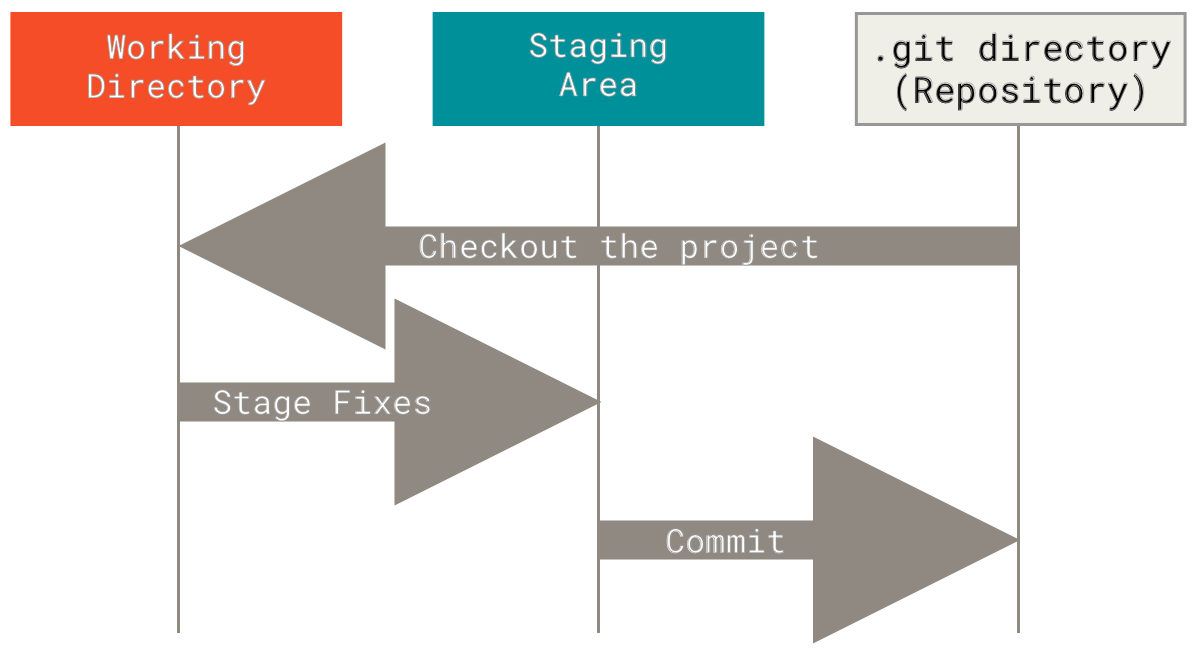
\includegraphics[width=75mm]{assets/official/collected/git-areas.png}}
  \DAtagline{关键路径}{\DAcmd{git add} 把变化送入暂存区；\DAcmd{git commit} 写入本地仓库}
  \DAsource{Pro Git · The Three States}{https://git-scm.com/book/en/v2/Getting-Started-What-is-Git\%3F}
\end{frame}

\begin{frame}[fragile]{2.2 第一次使用 Git 的身份配置}{作者信息会写入每个 Commit}
  \begin{lstlisting}[language=bash]
git config --global user.name "Your Name"
git config --global user.email "you@example.com"

git config --global init.defaultBranch main
git config --global --list
  \end{lstlisting}
  \begin{itemize}
    \item 公司与个人账号需要区分时，可在项目目录使用不带 \DAcmd{--global} 的配置。
    \item 提交邮箱应与 GitHub 账号关联，才能正确显示贡献身份。
    \item 认证使用 SSH Key 或受控 Token；密码与 Token 留在受控环境。
  \end{itemize}
\end{frame}

\begin{frame}[fragile]{2.3 获取仓库：init 与 clone}{一个创建新历史，一个复制已有历史}
  \begin{columns}[T]
    \begin{column}{0.48\textwidth}
      \begin{block}{新项目}
        \begin{lstlisting}[language=bash]
mkdir customer-service
cd customer-service
git init
git status
        \end{lstlisting}
      \end{block}
    \end{column}
    \begin{column}{0.48\textwidth}
      \begin{block}{已有项目}
        \begin{lstlisting}[language=bash]
git clone git@github.com:org/app.git
cd app
git remote -v
        \end{lstlisting}
      \end{block}
    \end{column}
  \end{columns}
  \DAtagline{团队默认}{使用 Clone 获取完整历史与远程仓库配置}
\end{frame}

\begin{frame}[fragile]{2.4 一次最小提交循环：从 git add 开始}{选择文件、检查暂存区、创建本地 Commit}
  \begin{columns}[T]
    \begin{column}{0.42\textwidth}
  \begin{lstlisting}[language=bash,basicstyle=\ttfamily\fontsize{5.4}{6.2}\selectfont]
git add docs/git-demo-notes.md
git diff --cached
git commit -m "docs: add Git workflow demo notes"
  \end{lstlisting}
      \begin{itemize}
        \item 先选择，再检查，最后提交。
        \item Commit 只写入本机仓库。
      \end{itemize}
    \end{column}
    \begin{column}{0.54\textwidth}
      \centering
      \DAframed{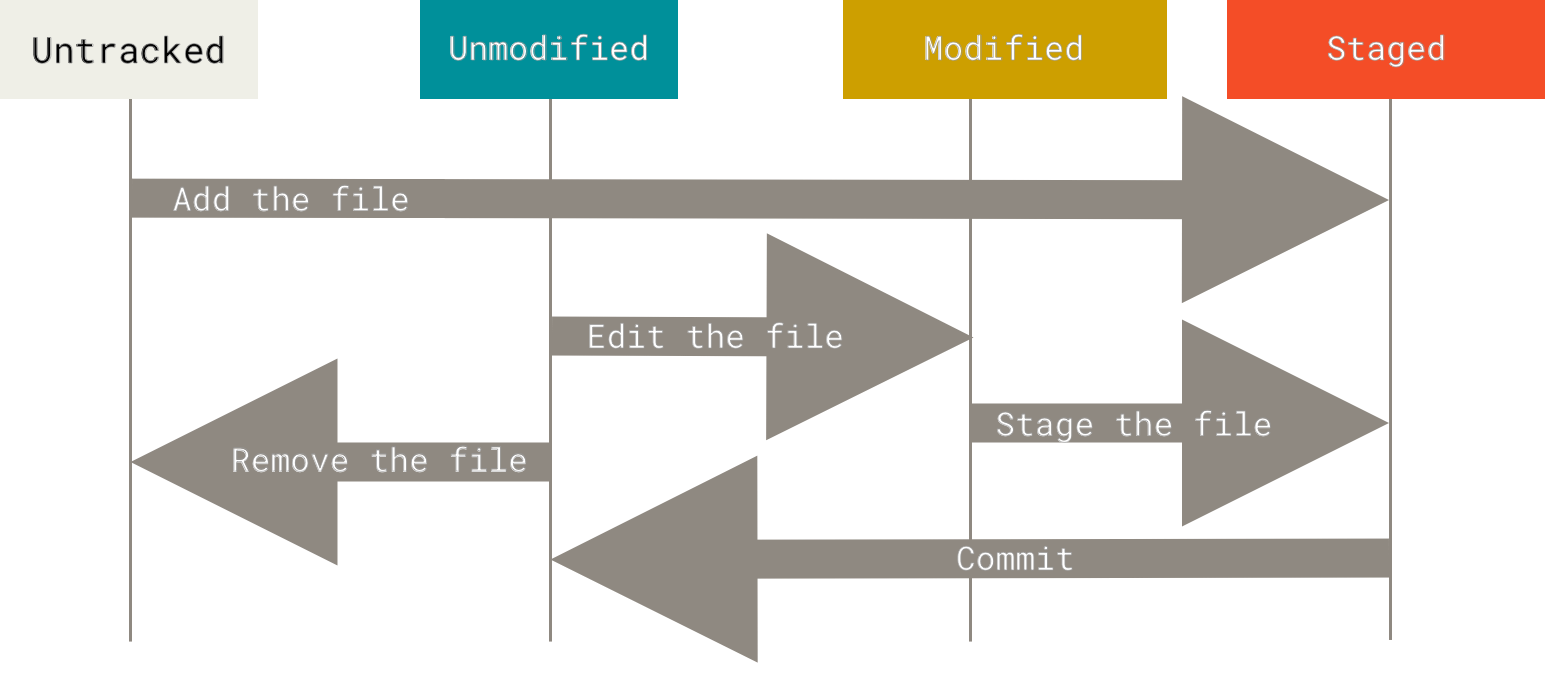
\includegraphics[width=66mm]{assets/official/collected/git-lifecycle.png}}
      \par\smallskip
      {\scriptsize 文件会在未跟踪、已修改、已暂存之间流转。}
    \end{column}
  \end{columns}
  \DAsource{Pro Git · Recording Changes}{https://git-scm.com/book/en/v2/Git-Basics-Recording-Changes-to-the-Repository}
\end{frame}

\begin{frame}[fragile]{2.5 Commit 写入本地仓库}{Commit 0fd229a}
  \begin{lstlisting}[language=bash]
$ git diff --cached --stat
 docs/git-demo-notes.md | 13 +++++++++++++
 1 file changed, 13 insertions(+)

$ git commit -m "docs: add Git workflow demo notes"
[main 0fd229a] docs: add Git workflow demo notes
 1 file changed, 13 insertions(+)
 create mode 100644 docs/git-demo-notes.md
  \end{lstlisting}
  \DAtagline{此刻}{Commit 已存在于本地，GitHub 仍停留在上一个 Commit}
\end{frame}

\begin{frame}[fragile]{2.6 Push 同步到 GitHub}{Commit 是本地动作，Push 是网络动作}
  \begin{columns}[T]
    \begin{column}{0.48\textwidth}
      \begin{block}{Push 前}
        \begin{lstlisting}[language=bash]
$ git status -sb
## main...origin/main [ahead 1]

$ git log --oneline --decorate -2
0fd229a (HEAD -> main) docs: add
  Git workflow demo notes
8ce893a (origin/main) feat: add
  deployment and operations lessons
        \end{lstlisting}
      \end{block}
    \end{column}
    \begin{column}{0.48\textwidth}
      \begin{block}{Push 后}
        \begin{lstlisting}[language=bash]
$ git push
 8ce893a..0fd229a  main -> main

$ git status -sb
## main...origin/main
        \end{lstlisting}
      \end{block}
    \end{column}
  \end{columns}
\end{frame}

\begin{frame}{2.7 好 Commit 的三个标准}{小、完整、能读懂}
  \begin{columns}[T]
    \begin{column}{0.52\textwidth}
      \begin{itemize}
        \item \textbf{单一意图}：一次只解决一个问题。
        \item \textbf{可独立验证}：提交后项目仍可运行或测试。
        \item \textbf{信息明确}：说明改了什么以及为什么改。
      \end{itemize}
      \DAtagline{示例}{\DAfile{fix(api): handle 401 response}}
    \end{column}
    \begin{column}{0.44\textwidth}
      \centering
      \DAframed{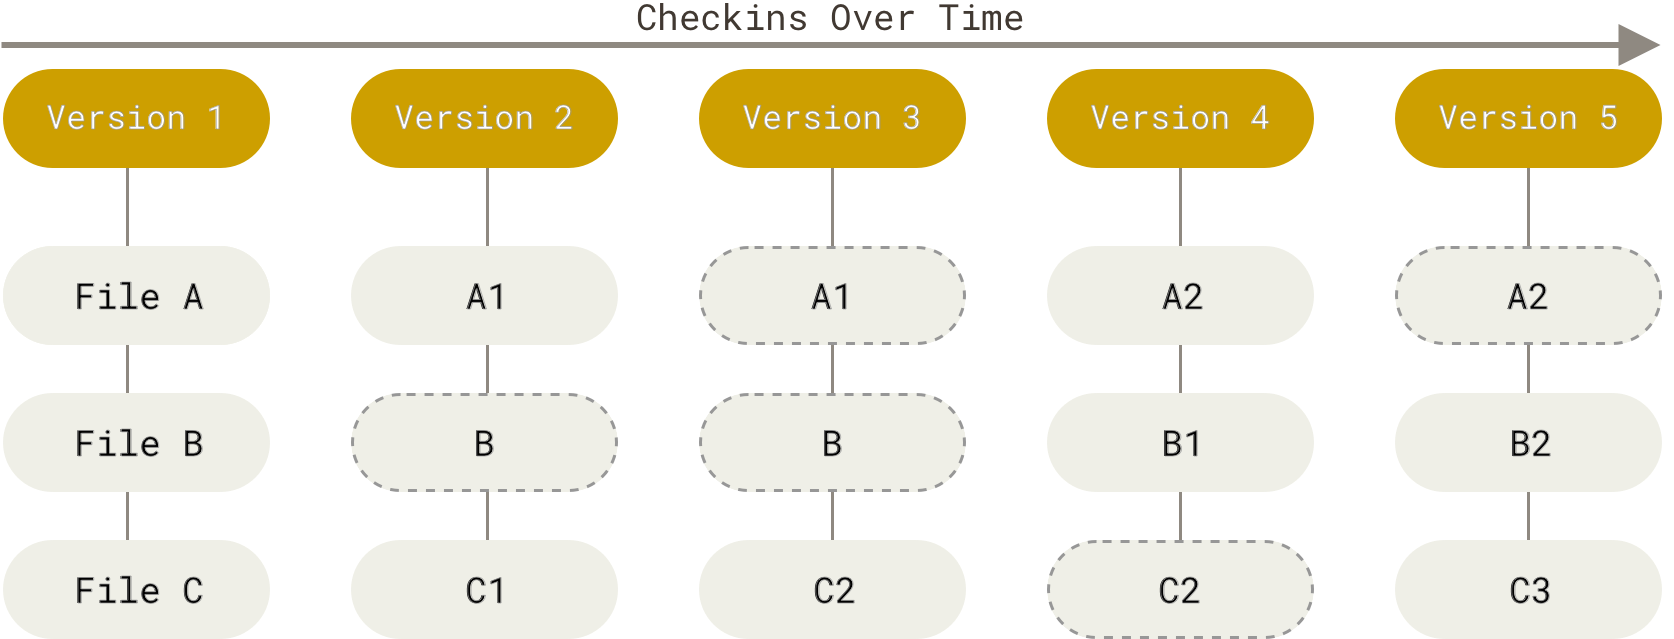
\includegraphics[width=53mm]{assets/official/collected/git-snapshots.png}}
      \par\smallskip
      {\scriptsize 每个 Commit 保存一次可追踪的项目快照。}
    \end{column}
  \end{columns}
  \DAsource{Pro Git · Snapshots, Not Differences}{https://git-scm.com/book/en/v2/Getting-Started-What-is-Git\%3F}
\end{frame}

\begin{frame}[fragile]{2.8 用 log 与 show 追踪变化}{查看提交顺序、指针位置与文件变化}
  \begin{lstlisting}[language=bash]
$ git log --oneline --decorate --graph -4
* 0fd229a (HEAD -> main, origin/main)
  docs: add Git workflow demo notes
* 8ce893a feat: add deployment and operations lessons
* bef37be feat: add Git collaboration lessons
* ab2afa2 chore: initialize Day 5 beamer project

$ git show --stat 0fd229a
 docs/git-demo-notes.md | 13 +++++++++++++
 1 file changed, 13 insertions(+)
  \end{lstlisting}
  \begin{itemize}
    \item \DAfile{HEAD -> main, origin/main} 表示本地与 GitHub 已对齐。
    \item \DAcmd{git show 0fd229a} 查看某次提交的说明与完整 Diff。
    \item \DAcmd{git diff ab2afa2..0fd229a} 比较两个历史节点。
  \end{itemize}
\end{frame}

\begin{frame}{2.9 分支是什么}{指向某个 Commit 的可移动标签}
  \centering
  \DAframed{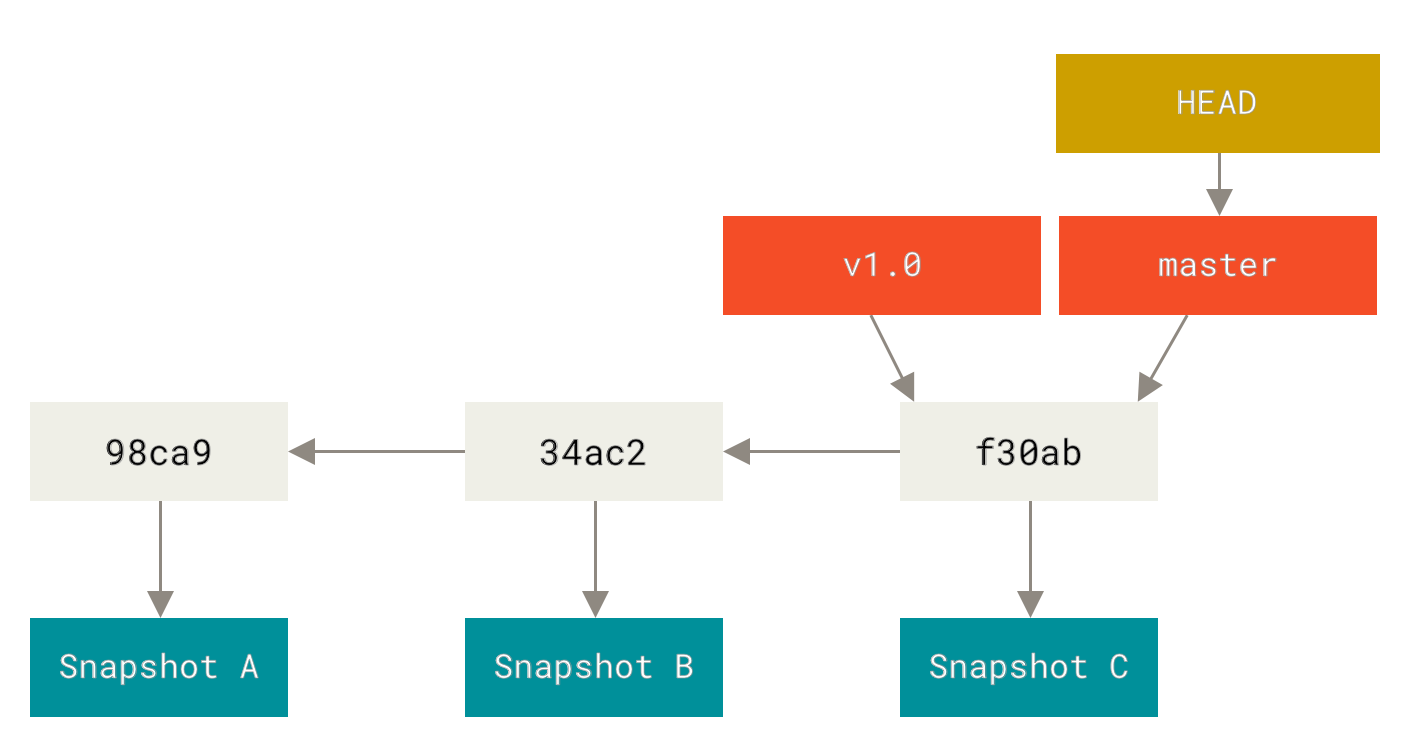
\includegraphics[width=70mm]{assets/official/collected/git-branch-history.png}}
  \begin{itemize}
    \item 分支是指向 Commit 的轻量指针。
    \item 每个任务独立分支，可以并行开发、单独 Review、随时放弃。
  \end{itemize}
  \DAsource{Pro Git · Branches in a Nutshell}{https://git-scm.com/book/en/v2/Git-Branching-Branches-in-a-Nutshell}
\end{frame}

\begin{frame}[fragile]{2.10 分支的日常命令}{从最新 main 开始工作}
  \begin{columns}[T]
    \begin{column}{0.53\textwidth}
  \begin{lstlisting}[language=bash,basicstyle=\ttfamily\fontsize{5.2}{6.0}\selectfont]
git switch main
git pull --ff-only

git switch -c feature/login-api
# edit, test, commit...

git switch main
git branch -d feature/login-api
  \end{lstlisting}
    \end{column}
    \begin{column}{0.43\textwidth}
      \centering
      \DAframed{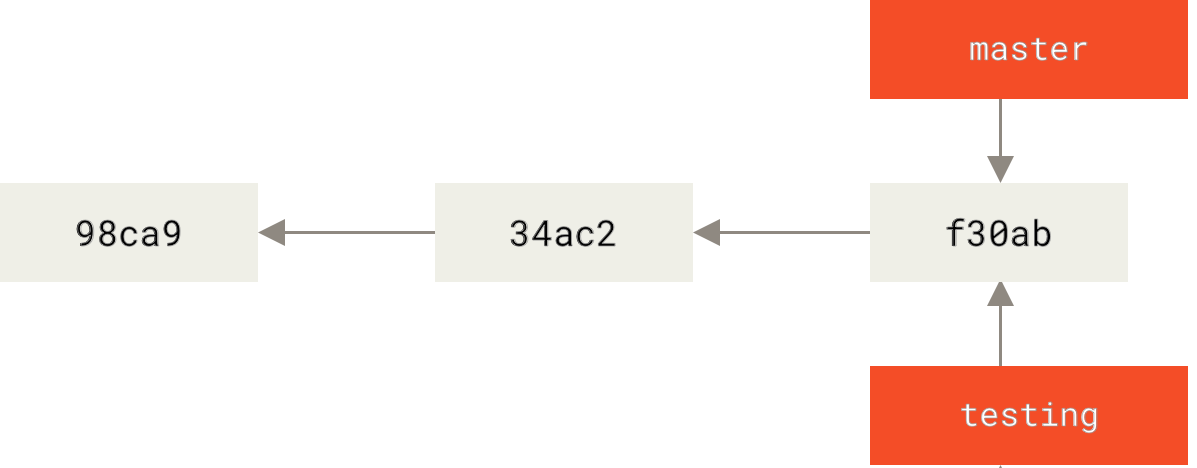
\includegraphics[width=52mm]{assets/official/collected/git-two-branches.png}}
      \begin{itemize}
        \item 从最新 \DAfile{main} 创建任务分支。
        \item 合并后及时删除过期分支。
      \end{itemize}
    \end{column}
  \end{columns}
  \DAsource{Pro Git · Basic Branching}{https://git-scm.com/book/en/v2/Git-Branching-Basic-Branching-and-Merging}
\end{frame}

\begin{frame}[fragile]{2.11 撤销操作：先判断“是否已经共享”}{公开历史优先 revert，未共享历史才考虑重写}
  \begin{DAtable*}{@{}p{29mm}p{45mm}p{47mm}@{}}
    \toprule
    场景 & 推荐命令 & 影响 \\
    \midrule
    未暂存的文件改坏 & \DAcmd{git restore file} & 丢弃本地变化 \\
    误加入暂存区 & \DAcmd{git restore --staged file} & 保留文件变化 \\
    最近 Commit 信息错 & \DAcmd{git commit --amend} & 重写未共享提交 \\
    已推送的错误 Commit & \DAcmd{git revert <commit>} & 新增反向提交，历史安全 \\
    \bottomrule
  \end{DAtable*}
  \DAtagline{红线}{共享分支不执行 \DAcmd{reset --hard} 或普通 \DAcmd{push --force}}
\end{frame}

\DAsection[分支负责隔离，Pull Request 负责让变化被看见、被讨论、被批准]{GitHub 团队协作工作流}

\begin{frame}{3.1 两种常见协作模型}{同仓库分支适合内部团队，Fork 适合外部贡献}
  \begin{columns}[T]
    \begin{column}{0.48\textwidth}
      \begin{block}{Shared Repository}
        \begin{itemize}
          \item 成员对同一仓库有写权限
          \item 每人创建 Topic Branch
          \item PR 合并回 \DAfile{main}
          \item 适合课程小组、公司内部项目
        \end{itemize}
      \end{block}
    \end{column}
    \begin{column}{0.48\textwidth}
      \begin{block}{Fork + Pull Request}
        \begin{itemize}
          \item 贡献者在自己的 Fork 中修改
          \item 向上游仓库发起 PR
          \item 通过 Fork 向上游提交变更
          \item 适合开源、外部合作方
        \end{itemize}
      \end{block}
    \end{column}
  \end{columns}
  \DAtagline{课程选择}{优先使用 Shared Repository，减少初学阶段的 remote / upstream 复杂度}
\end{frame}

\begin{frame}{3.2 从需求到代码：先拆任务，再建分支}{一个分支对应一个独立工作单元}
  \centering
  \begin{tikzpicture}[node distance=2mm]
    \node[DAflow,minimum width=18mm] (issue) {Issue\\定义问题};
    \node[DAflow,minimum width=18mm,right=of issue] (owner) {Assign\\负责人};
    \node[DAflow,minimum width=18mm,right=of owner] (branch) {Branch\\隔离};
    \node[DAflow,minimum width=18mm,right=of branch] (commit) {Commit\\记录};
    \node[DAflow,minimum width=18mm,right=of commit] (pr) {PR\\审查};
    \node[DAflow,minimum width=18mm,right=of pr] (done) {Merge\\完成};
    \draw[DAarrowred] (issue) -- (owner);
    \draw[DAarrowred] (owner) -- (branch);
    \draw[DAarrowred] (branch) -- (commit);
    \draw[DAarrowred] (commit) -- (pr);
    \draw[DAarrowred] (pr) -- (done);
  \end{tikzpicture}
  \par\medskip
  \begin{itemize}
    \item Issue 写清背景、范围、完成条件与边界。
    \item 分支名带任务语义；PR 描述中关联 Issue。
    \item 一个分支只服务一个目标，减少冲突与 Review 负担。
  \end{itemize}
\end{frame}

\begin{frame}[fragile]{3.3 开发者的完整命令流}{同步、建分支、提交、推送}
  \begin{lstlisting}[language=bash]
git switch main
git pull --ff-only
git switch -c feature/chat-history

# edit and test
git status
git diff
git add src/
git commit -m "feat(chat): load conversation history"

git push -u origin feature/chat-history
  \end{lstlisting}
  \DAtagline{关键动作}{首次 push 后立即创建 Pull Request}
\end{frame}

\begin{frame}{3.4 Pull Request：提交变更提案}{base 是要进入的分支，compare 是你的分支}
  \centering
  \DAframed{
\includegraphics[width=111mm]{assets/official/github-compare-pr.png}}
  \begin{itemize}
    \item 标题说明结果，正文解释背景、方案、测试证据与风险。
    \item Draft PR 可尽早暴露方向，避免做完才发现设计不对。
    \item PR 后续新增 Commit 会自动进入同一个审查上下文。
  \end{itemize}
  \DAsource{GitHub Docs · Creating a pull request}{https://docs.github.com/en/pull-requests/collaborating-with-pull-requests/proposing-changes-to-your-work-with-pull-requests/creating-a-pull-request}
\end{frame}

\begin{frame}{3.5 一个合格 PR 描述应该包含什么}{让 Review 者快速理解}
  \begin{columns}[T]
    \begin{column}{0.48\textwidth}
      \begin{block}{建议模板}
        \begin{itemize}
          \item \textbf{Why}：为什么要改
          \item \textbf{What}：核心改动
          \item \textbf{How to test}：如何验证
          \item \textbf{Screenshots}：界面证据
          \item \textbf{Risk / rollback}：风险与回滚
        \end{itemize}
      \end{block}
    \end{column}
    \begin{column}{0.48\textwidth}
      \begin{alertblock}{避免}
        \begin{itemize}
          \item “改好了，请看”
          \item 没有说明数据库迁移
          \item 没有列环境变量变化
          \item 把多个不相关任务塞进一个 PR
          \item 自己都没打开 Files changed
        \end{itemize}
      \end{alertblock}
    \end{column}
  \end{columns}
\end{frame}

\begin{frame}{3.6 Code Review 看什么}{先看正确性和风险，再看风格}
  \centering
  \DAframed{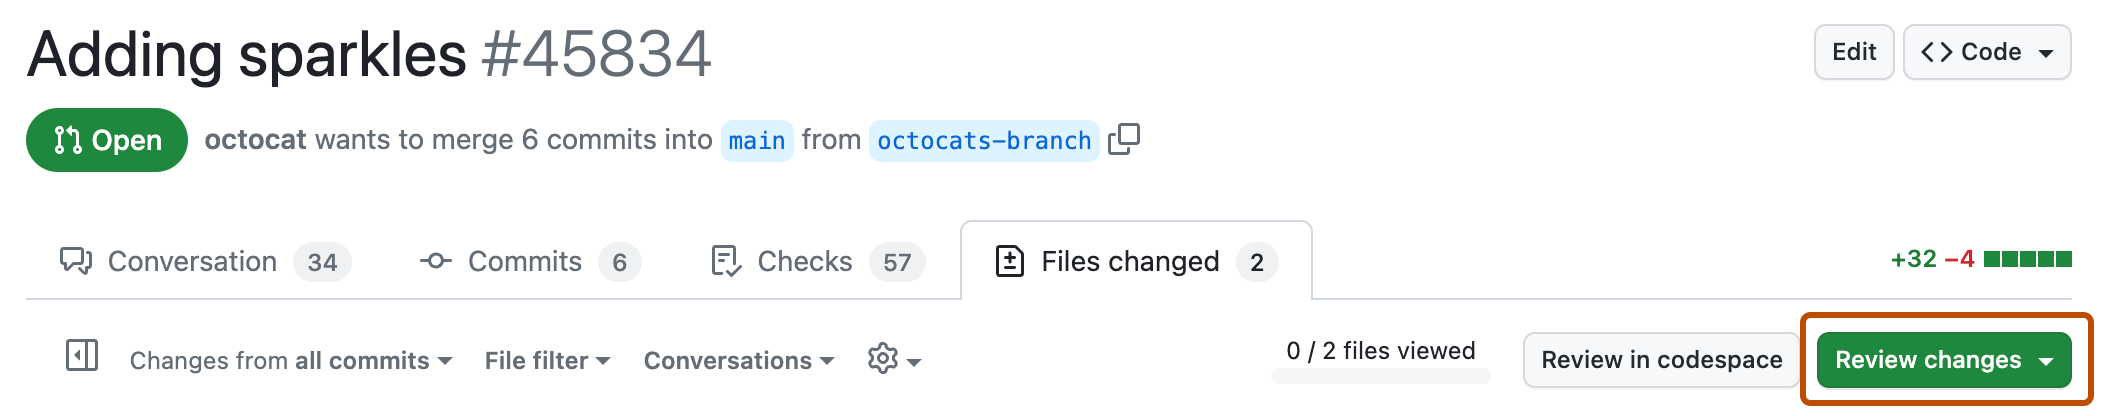
\includegraphics[width=119mm]{assets/official/github-review-changes.png}}
  \begin{itemize}
    \item 需求是否真的满足？边界条件、错误处理、权限校验是否完整？
    \item 是否引入密钥、调试代码、重复逻辑或破坏兼容性？
    \item Review 结论：Comment、Approve、Request changes。
  \end{itemize}
  \DAsource{GitHub Docs · Reviewing proposed changes}{https://docs.github.com/en/pull-requests/collaborating-with-pull-requests/reviewing-changes-in-pull-requests/reviewing-proposed-changes-in-a-pull-request}
\end{frame}

\begin{frame}{3.7 Review 评论要对事、可执行}{指出风险，也给出下一步}
  \begin{DAtable}{@{}p{34mm}p{83mm}@{}}
    \toprule
    评论类型 & 示例 \\
    \midrule
    阻塞问题 & 这里把用户 ID 直接相信前端传值，会产生越权，请从 Token 读取身份。 \\
    建议改进 & 建议把重复的请求逻辑提取到 API Client；本 PR 不阻塞，可另开任务。 \\
    澄清问题 & 这里为何选择 204？前端是否读取响应正文？ \\
    肯定反馈 & 这个错误结构与现有接口一致，前端处理会更简单。 \\
    \bottomrule
  \end{DAtable}
  \DAtagline{团队文化}{Review 代码，不评价人；问题要具体到行为、风险与验证方式}
\end{frame}

\begin{frame}{3.8 三种合并方式怎么选}{小团队建议默认 Squash merge}
  \begin{DAtable}{@{}p{28mm}p{43mm}p{48mm}@{}}
    \toprule
    方式 & 历史结果 & 适用场景 \\
    \midrule
    Merge commit & 保留分支与所有 Commit & 需要完整分支拓扑 \\
    Squash merge & PR 压成一个 Commit & 功能分支过程较碎，小团队默认 \\
    Rebase merge & 每个 Commit 线性接到 main & Commit 本身质量高、团队熟悉 Rebase \\
    \bottomrule
  \end{DAtable}
  \begin{itemize}
    \item 规则要统一，否则历史一会儿分叉、一会儿线性，回滚与排查更难。
    \item Squash 后 PR 标题应成为高质量 Commit 信息。
  \end{itemize}
\end{frame}

\begin{frame}[fragile]{3.9 PR 开发期间如何同步 main}{降低最终合并时的冲突}
  \begin{columns}[T]
    \begin{column}{0.48\textwidth}
      \begin{block}{Merge main}
        \begin{lstlisting}[language=bash]
git fetch origin
git switch feature/chat-history
git merge origin/main
        \end{lstlisting}
        \scriptsize 保留真实分叉关系，不重写已有 Commit。
      \end{block}
    \end{column}
    \begin{column}{0.48\textwidth}
      \begin{block}{Rebase onto main}
        \begin{lstlisting}[language=bash]
git fetch origin
git switch feature/chat-history
git rebase origin/main
        \end{lstlisting}
        \scriptsize 历史更线性，但会重写分支 Commit ID。
      \end{block}
    \end{column}
  \end{columns}
  \DAtagline{约定}{初学团队优先 Merge；熟悉 Rebase 后由团队统一切换}
\end{frame}

\begin{frame}{3.10 密钥必须留在 Git 之外}{泄漏后立即轮换并清理历史}
  \begin{alertblock}{严禁提交}
    \DAfile{.env}、数据库密码、JWT Secret、云厂商密钥、模型 API Key、私钥文件。
  \end{alertblock}
  \begin{itemize}
    \item 发现泄漏后立即吊销或轮换密钥，再处理仓库文件。
    \item 再清理 Git 历史、检查 Fork / 缓存 / CI 日志，并复盘为何未被拦截。
    \item 部署时通过服务器环境变量、Secret 文件或平台 Secret 注入。
  \end{itemize}
  \DAtagline{提交前检查}{\DAcmd{git diff --staged} + Secret Scanner + 最小权限密钥}
\end{frame}

\DAsection[读标记、解冲突、保护 main]{冲突处理、Review 与主分支治理}

\begin{frame}[fragile]{4.1 先学会读冲突标记}{当前分支、分隔线、待合并分支}
  \centering
  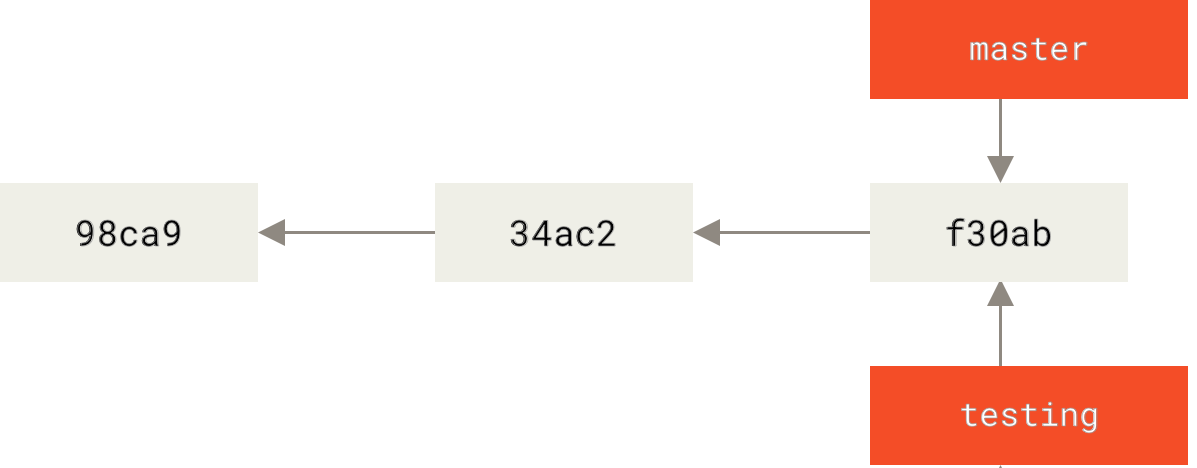
\includegraphics[width=48mm]{assets/official/collected/git-two-branches.png}
  \begin{lstlisting}
<<<<<<< HEAD
const apiBase = "/api";
=======
const apiBase = "http://localhost:8000";
>>>>>>> feature/api-config
  \end{lstlisting}
  \begin{itemize}
    \item 先确认生产架构与配置约定，再选择或融合两侧代码。
    \item 删除全部标记后，必须重新运行测试与构建。
  \end{itemize}
  \DAsource{Pro Git · Divergent Branches}{https://git-scm.com/book/en/v2/Git-Branching-Branches-in-a-Nutshell}
\end{frame}

\begin{frame}[fragile]{4.2 命令行解决冲突的标准步骤}{定位、编辑、验证、继续}
  \begin{lstlisting}[language=bash]
git status
# open conflicted files and resolve markers

pnpm lint
pnpm test
pnpm build

git add src/config/api.ts
git commit                 # merge workflow
# or: git rebase --continue
  \end{lstlisting}
  \begin{itemize}
    \item \DAcmd{git status} 会列出所有未合并路径。
    \item 不确定时可用 \DAcmd{git merge --abort} 或 \DAcmd{git rebase --abort} 回到操作前。
    \item 解决冲突时必须理解两边业务意图。
  \end{itemize}
\end{frame}

\begin{frame}{4.3 GitHub 在线解决简单行冲突}{复杂冲突回到本地测试}
  \centering
  \DAframed{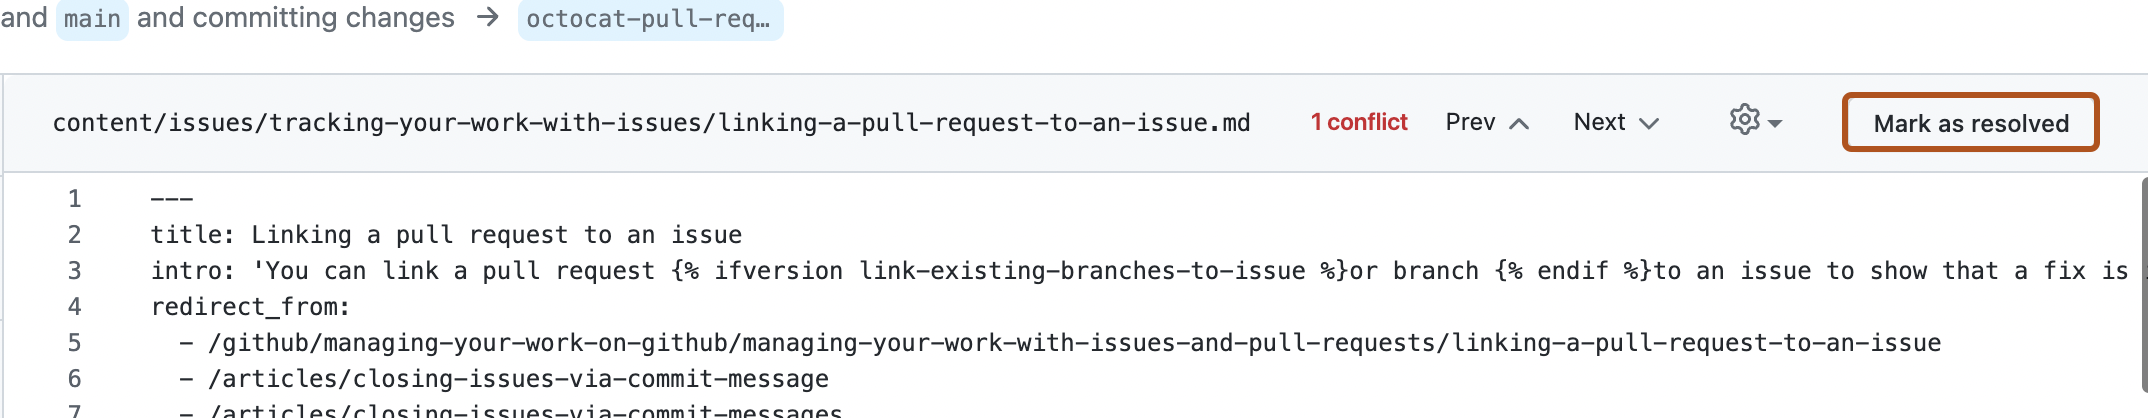
\includegraphics[width=119mm]{assets/official/github-conflict-editor.png}}
  \begin{itemize}
    \item 简单的竞争行可以使用网页冲突编辑器。
    \item 删除 / 重命名、生成文件、依赖锁文件等复杂冲突建议本地处理。
    \item 合并前必须验证构建、测试和关键业务流程。
  \end{itemize}
  \DAsource{GitHub Docs · Resolving a merge conflict}{https://docs.github.com/en/pull-requests/collaborating-with-pull-requests/addressing-merge-conflicts/resolving-a-merge-conflict-on-github}
\end{frame}

\begin{frame}{4.4 如何减少冲突}{重点是工作拆分、同步和接口约定}
  \begin{columns}[T]
    \begin{column}{0.54\textwidth}
      \begin{itemize}
        \item 拆成小任务，使用短生命周期分支。
        \item 明确模块负责人，减少同时修改核心文件。
        \item 频繁同步 \DAfile{main}，尽早暴露竞争变化。
        \item Schema、路由和公共配置先约定再编码。
        \item 格式化与依赖更新单独提交。
      \end{itemize}
    \end{column}
    \begin{column}{0.42\textwidth}
      \centering
      \DAframed{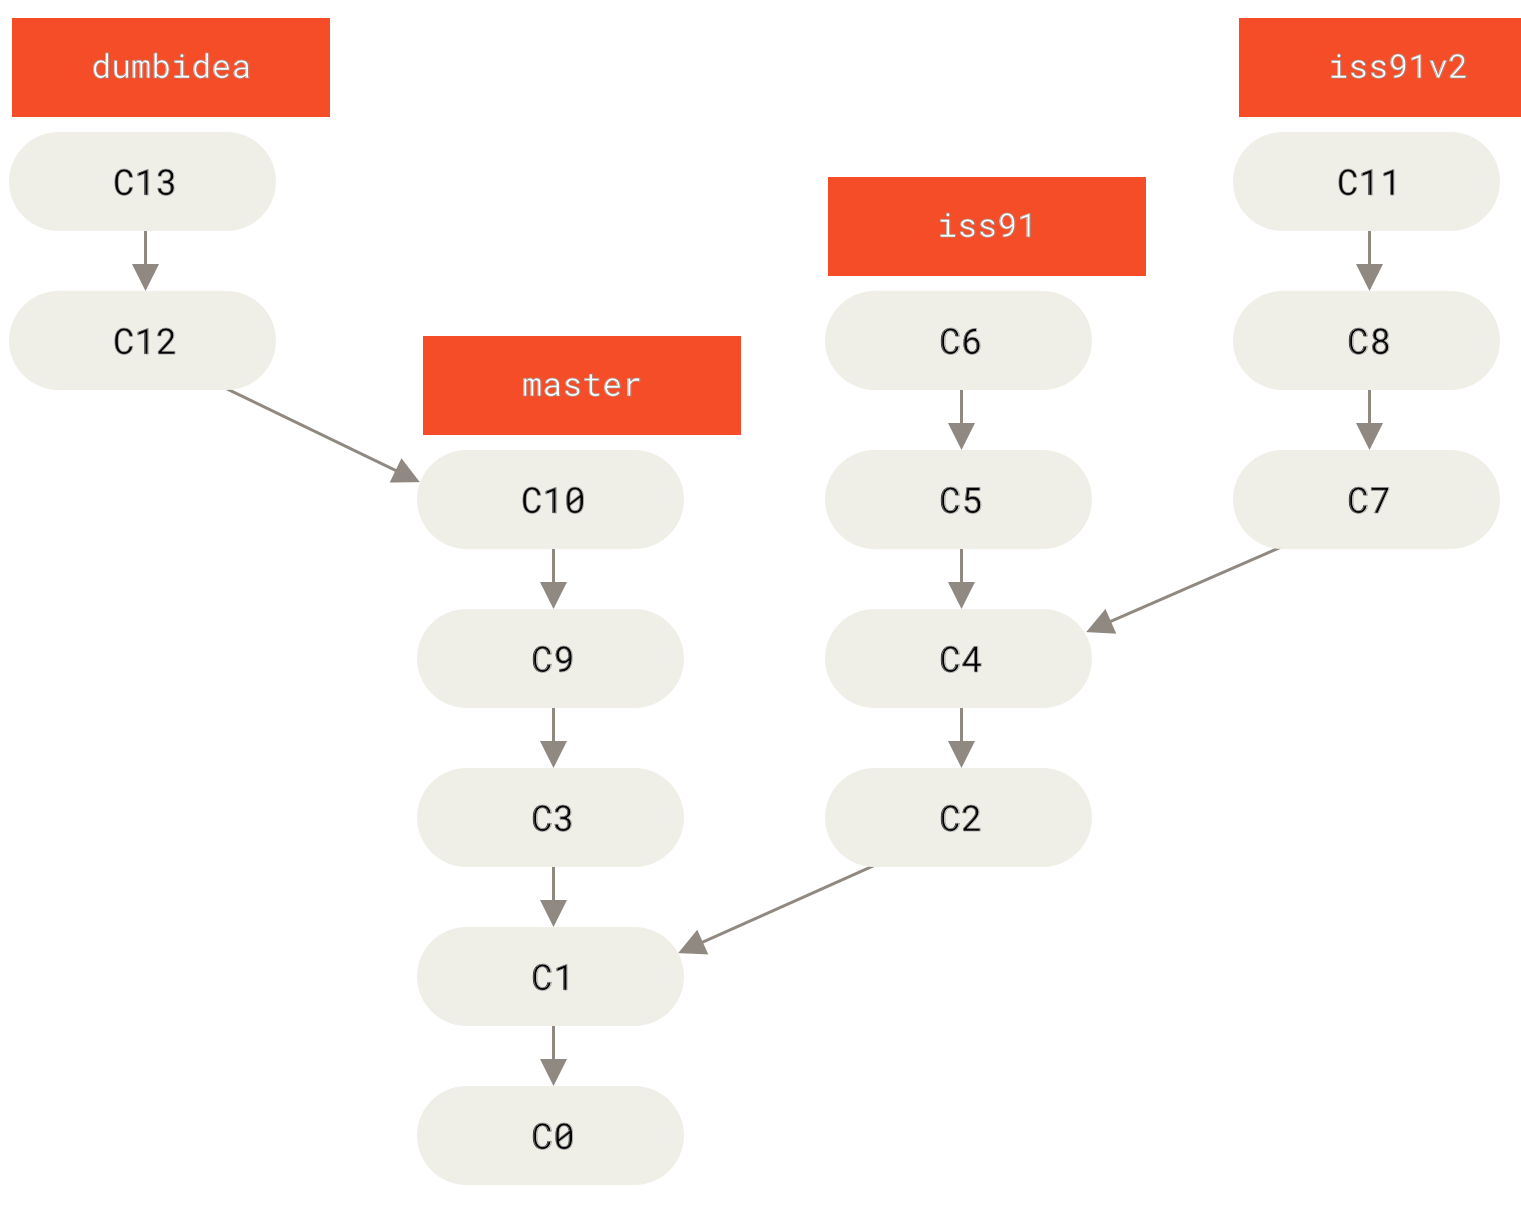
\includegraphics[width=46mm]{assets/official/collected/git-topic-branches.png}}
      \par\smallskip
      {\scriptsize 一个分支只承载一个清晰任务。}
    \end{column}
  \end{columns}
  \DAsource{Pro Git · Topic Branches}{https://git-scm.com/book/en/v2/Git-Branching-Branching-Workflows}
\end{frame}

\begin{frame}{4.5 Rebase 为什么需要谨慎}{它会把 Commit 复制到新的父节点上}
  \centering
  \DAframed{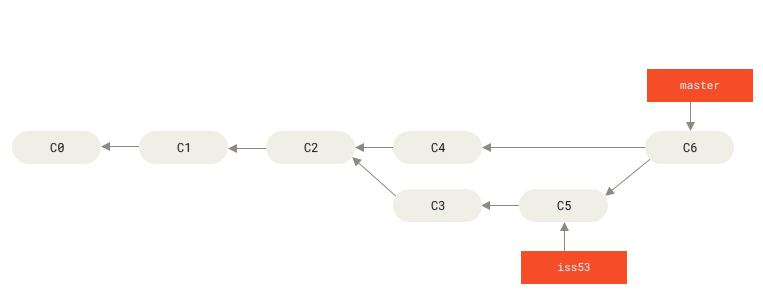
\includegraphics[width=84mm]{assets/official/collected/git-basic-merge.png}}
  \begin{itemize}
    \item Merge 保留分叉历史；Rebase 会复制提交到新的父节点。
    \item Rebase 后 Commit ID 改变，远程推送可能需要历史重写。
    \item 只重写自己的功能分支；共享历史保持稳定。
  \end{itemize}
  \DAsource{Pro Git · Basic Merging}{https://git-scm.com/book/en/v2/Git-Branching-Basic-Branching-and-Merging}
\end{frame}

\begin{frame}[fragile]{4.6 Rebase 后推送用 force-with-lease}{它会检查远程分支是否被别人更新}
  \begin{lstlisting}[language=bash]
git fetch origin
git rebase origin/main

git push --force-with-lease
  \end{lstlisting}
  \begin{alertblock}{禁止使用}
    \DAcmd{git push --force} 可能覆盖同事刚推送的 Commit。
  \end{alertblock}
  \DAtagline{边界}{如果团队尚未理解历史重写，统一用 Merge 同步 main 更安全}
\end{frame}

\begin{frame}{4.7 主分支保护规则}{main 始终代表“可部署版本”}
  \begin{itemize}
    \item 禁止直接 Push，所有变化通过受控合并流程进入 \DAfile{main}。
    \item 至少一人 Approve，关键目录可配置 CODEOWNERS。
    \item 必须通过构建、测试、Lint 等状态检查。
    \item 必须解决 Review 对话后才能合并。
    \item 默认禁止 Force Push 与删除主分支。
  \end{itemize}
  \DAtagline{结果}{规则把“团队口头约定”变成平台自动执行的门禁}
  \DAsource{GitHub Docs · About protected branches}{https://docs.github.com/en/repositories/configuring-branches-and-merges-in-your-repository/managing-protected-branches/about-protected-branches}
\end{frame}

\DAsection[公网入口、端口与部署路线]{服务器购买占位与部署架构}

\begin{frame}{5.1 服务器购买 · 现场演示}{购买页由讲师现场操作}
  \begin{columns}[T]
    \begin{column}{0.46\textwidth}
      \DAtagline{地域}{靠近用户；境内上线关注备案}
      \DAtagline{系统}{Ubuntu / Debian LTS 纯净镜像}
      \DAtagline{配置}{课堂建议 2C4G 起步}
      \DAtagline{网络}{公网 IPv4、带宽、22 / 80 / 443}
    \end{column}
    \begin{column}{0.50\textwidth}
      \DAfigureph[34mm]{现场演示：购买服务器\\记录公网 IP 与登录方式}
      \DAtagline*{提醒}{在中国境内提供互联网信息服务，应依法判断备案 / 许可要求}
    \end{column}
  \end{columns}
  \DAsource{工信部 · 非经营性互联网信息服务备案管理办法}{https://www.miit.gov.cn/api-gateway/jpaas-web-server/front/document/file-download?fileName=f1b8d119f55240b4813dd39360d2e0b0.pdf}
\end{frame}

\begin{frame}{5.2 公网请求路径}{DNS、Nginx、前端、API 与数据库}
  \centering
  \begin{tikzpicture}[node distance=2mm]
    \node[DAflow,minimum width=18mm] (dns) {DNS\\域名解析};
    \node[DAflow,minimum width=18mm,right=of dns] (firewall) {云防火墙\\80 / 443};
    \node[DAflow,minimum width=18mm,right=of firewall] (nginx) {Nginx\\TLS};
    \node[DAflow,minimum width=18mm,right=of nginx] (front) {前端\\静态 / SSR};
    \node[DAflow,minimum width=18mm,right=of front] (api) {API\\127.0.0.1};
    \node[DAstore,right=of api] (db) {MySQL};
    \draw[DAarrowred] (dns) -- (firewall);
    \draw[DAarrowred] (firewall) -- (nginx);
    \draw[DAarrowred] (nginx) -- (front);
    \draw[DAarrowred] (front) -- node[above,font=\tiny]{/api} (api);
    \draw[DAarrow] (api) -- (db);
  \end{tikzpicture}
  \par\medskip
  \begin{itemize}
    \item 公网只开放必要入口；8000、3000、3306 留在本机或容器网络。
    \item Nginx 负责域名、HTTPS、静态文件与反向代理。
  \end{itemize}
\end{frame}

\begin{frame}{5.3 端口开放策略}{公网保留 22、80、443}
  \begin{DAtable}{@{}p{19mm}p{37mm}p{67mm}@{}}
    \toprule
    端口 & 典型用途 & 建议 \\
    \midrule
    22 & SSH & 仅管理使用；可限制来源 IP、使用密钥登录 \\
    80 & HTTP & 证书验证与跳转 HTTPS \\
    443 & HTTPS & 用户正式访问入口 \\
    3000 & Node / Next.js & 默认仅本机或容器网络 \\
    8000 & FastAPI & 默认仅本机或容器网络 \\
    3306 & MySQL & 不向公网开放，应用走本机 / 内网 \\
    \bottomrule
  \end{DAtable}
  \DAsource{阿里云轻量应用服务器 · 防火墙}{https://help.aliyun.com/zh/simple-application-server/user-guide/manage-the-firewall-of-a-server}
\end{frame}

\begin{frame}{5.4 宝塔与 Docker 的分工}{可视化运维与可重复交付}
  \begin{DAtable}{@{}p{24mm}p{47mm}p{48mm}@{}}
    \toprule
    维度 & 宝塔部署 & Docker 部署 \\
    \midrule
    学习门槛 & 面板可视化，上手快 & 需要理解镜像、网络、卷 \\
    环境一致性 & 依赖服务器当前状态 & 镜像描述运行环境 \\
    迁移复现 & 需要记录手工步骤 & Dockerfile + Compose 可重复 \\
    排错入口 & 面板日志 + 系统日志 & docker logs + 容器状态 \\
    适用 & 新手、小型单机项目 & 团队交付、多服务、持续迭代 \\
    \bottomrule
  \end{DAtable}
  \DAtagline{组合方式}{宝塔管理 Nginx 与证书，Docker Compose 运行应用}
\end{frame}

\DAsection[用面板管理 Nginx、进程、数据库与证书]{通过宝塔部署全栈项目}

\begin{frame}{6.1 安装宝塔后的第一件事：加固面板}{面板是高权限管理入口}
  \begin{enumerate}
    \item 从宝塔官网复制当前系统对应的官方安装命令。
    \item 保存安装输出中的面板地址、初始用户名和密码。
    \item 首次登录立即修改强密码、面板端口与安全入口。
    \item 云防火墙限制面板端口来源，优先绑定固定管理 IP。
    \item 开启面板 HTTPS、登录告警与必要的双因素验证。
  \end{enumerate}
  \begin{alertblock}{供应链提醒}
    不使用“破解版 / 纯净版 / 开心版”等第三方修改包，只从官方渠道安装与更新。
  \end{alertblock}
  \DAsource{宝塔官方下载}{https://www.bt.cn/new/download}
\end{frame}

\begin{frame}{6.2 安装基础环境}{Nginx、Node、pnpm、Python 与 MySQL}
  \begin{DAtable}{@{}p{28mm}p{38mm}p{55mm}@{}}
    \toprule
    组件 & 用途 & 选择建议 \\
    \midrule
    Nginx & 80 / 443、静态文件、反向代理 & 必装 \\
    Node.js & 构建前端、运行 Node 后端 / SSR & 安装项目要求的 LTS 版本 \\
    pnpm & Node 依赖与构建 & 通过 Corepack 或官方方式启用 \\
    Python + uv & FastAPI 运行环境 & 与 \DAfile{pyproject.toml} 要求一致 \\
    MySQL & 业务数据 & 本机部署时仅监听本地 / 内网 \\
    \bottomrule
  \end{DAtable}
  \vspace{1mm}
  {\small\textcolor{DARed}{\bfseries 原则：}项目版本来自仓库声明，生产升级要有计划。}
\end{frame}

\begin{frame}[fragile]{6.3 服务器获取代码的推荐方式}{Git Clone + 只读 Deploy Key}
  \begin{lstlisting}[language=bash]
cd /www/wwwroot
git clone git@github.com:your-org/customer-service.git
cd customer-service

git switch main
git pull --ff-only
git rev-parse --short HEAD
  \end{lstlisting}
  \begin{itemize}
    \item 服务器只负责部署时，Deploy Key 尽量设为只读。
    \item 记录当前 Commit ID，后续更新与回滚都以它为坐标。
    \item 不在服务器直接改业务代码，否则 Git 历史与线上状态会分叉。
  \end{itemize}
\end{frame}

\begin{frame}[fragile]{6.4 构建 Node 前端}{依赖锁定，API 地址使用生产配置}
  \begin{lstlisting}[language=bash]
cd /www/wwwroot/customer-service/frontend

corepack enable
pnpm install --frozen-lockfile
pnpm build

ls -la dist
  \end{lstlisting}
  \begin{itemize}
    \item Vite 常见输出目录是 \DAfile{dist/}；其他框架以项目配置为准。
    \item 推荐前端请求相对路径 \DAfile{/api}，由 Nginx 转发到后端。
    \item 构建时环境变量会写入静态文件，修改后必须重新构建。
  \end{itemize}
\end{frame}

\begin{frame}{6.5 创建静态站点}{网站根目录指向构建产物}
  \begin{enumerate}
    \item 宝塔左侧进入“网站”，添加站点并填写域名。
    \item 站点类型选择纯静态；根目录指向前端 \DAfile{dist/}。
    \item 确认运行用户对目录有读取权限。
    \item 暂时可用 HTTP 验证首页资源是否正确加载。
    \item 浏览器 F12 检查 HTML、JS、CSS 是否全部 200。
  \end{enumerate}
  \DAtagline{网站根目录}{只指向 \DAfile{dist/} 等生产构建产物}
  \DAsource{宝塔官方文档 · 添加站点}{https://docs.bt.cn/user-guide/site/php/create-web}
\end{frame}

\begin{frame}[fragile]{6.6 SPA 刷新 404 怎么修}{让未知前端路由回到 index.html}
  \begin{lstlisting}[language=bash]
location / {
    try_files $uri $uri/ /index.html;
}
  \end{lstlisting}
  \begin{itemize}
    \item React Router / Vue Router 的 History 模式由浏览器管理路由。
    \item 用户直接访问 \DAfile{/chat/123} 时，Nginx 找不到同名文件会返回 404。
    \item \DAcmd{try\_files} 让前端路由接管；\DAfile{/api} 保持独立代理规则。
  \end{itemize}
\end{frame}

\begin{frame}[fragile]{6.7 准备 FastAPI 生产环境}{服务器按锁文件创建独立虚拟环境}
  \begin{lstlisting}[language=bash]
cd /www/wwwroot/customer-service/backend

uv sync --locked --no-dev
uv run python -m pytest

uv run fastapi run app/main.py \
  --host 127.0.0.1 --port 8000 --proxy-headers
  \end{lstlisting}
  \begin{itemize}
    \item 先前台启动并用 \DAcmd{curl http://127.0.0.1:8000/health} 验证。
    \item 监听 \DAfile{127.0.0.1}，业务端口只允许本机 Nginx 访问。
    \item 确认无误后再交给宝塔项目管理 / 应用管理器守护。
  \end{itemize}
\end{frame}

\begin{frame}{6.8 FastAPI 进程守护}{SSH 断开后仍运行，异常后能重启}
  \begin{DAtable*}{@{}p{31mm}p{84mm}@{}}
    \toprule
    配置项 & 示例 \\
    \midrule
    项目目录 & \DAfile{/www/wwwroot/customer-service/backend} \\
    Python 环境 & 项目 \DAfile{.venv} 中的 Python / FastAPI \\
    启动命令 & 使用上一页命令，监听 \DAfile{127.0.0.1:8000} \\
    运行用户 & 非 root，确保能读代码与写日志 / 上传目录 \\
    环境变量 & 通过面板项目配置或受控 Env 文件注入 \\
    重启策略 & 开机启动、异常退出自动重启 \\
    \bottomrule
  \end{DAtable*}
  \DAtagline*{版本差异}{不同宝塔版本入口可能显示为 Python 项目、应用管理器或进程守护}
\end{frame}

\begin{frame}[fragile]{6.9 Nginx 把 /api 转给 FastAPI}{同域部署减少 CORS 与 Cookie 问题}
  \begin{lstlisting}[language=bash]
location /api/ {
    proxy_pass http://127.0.0.1:8000/;
    proxy_set_header Host $host;
    proxy_set_header X-Real-IP $remote_addr;
    proxy_set_header X-Forwarded-For $proxy_add_x_forwarded_for;
    proxy_set_header X-Forwarded-Proto $scheme;
}
  \end{lstlisting}
  \begin{itemize}
    \item 访问 \DAfile{https://app.example.com/api/health}，Nginx 转给 FastAPI。
    \item 注意 \DAcmd{proxy\_pass} 末尾斜杠会影响路径改写，必须现场验证真实路由。
    \item 后端启用 Proxy Headers 后，才能正确感知外部协议与客户端信息。
  \end{itemize}
  \DAsource{NGINX Docs · Reverse Proxy}{https://docs.nginx.com/nginx/admin-guide/web-server/reverse-proxy/}
\end{frame}

\begin{frame}{6.10 宝塔反向代理界面}{面板字段与 Nginx 配置一一对应}
  \begin{columns}[T]
    \begin{column}{0.42\textwidth}
      \begin{itemize}
        \item 代理名称：\DAfile{fastapi-api}
        \item 代理目录：\DAfile{/api/}
        \item 目标 URL：\DAfile{http://127.0.0.1:8000}
        \item 发送域名：通常使用 \DAfile{\$host}
        \item API 默认关闭缓存
      \end{itemize}
    \end{column}
    \begin{column}{0.54\textwidth}
      \centering
      \DAframed{
\includegraphics[width=68mm]{assets/official/bt-add-reverse-proxy.png}}
    \end{column}
  \end{columns}
  \DAsource{宝塔官方文档 · 反向代理}{https://docs.bt.cn/user-guide/site/php/site-config/reverse-proxy}
\end{frame}

\begin{frame}{6.11 前后端联调的验证顺序}{后端、Nginx、浏览器逐层检查}
  \begin{enumerate}
    \item \DAcmd{curl http://127.0.0.1:8000/health}：后端进程是否正常。
    \item \DAcmd{curl -i http://127.0.0.1/api/health}：Nginx 反代是否正常。
    \item 浏览器打开域名：前端静态资源是否正常。
    \item F12 Network 查看 \DAfile{/api/...} 请求、状态码、响应体。
    \item 后端日志确认同一请求是否到达、耗时与错误。
  \end{enumerate}
  \DAtagline{定位法}{在哪一层第一次失败，问题就位于该层或它的下一跳}
\end{frame}

\begin{frame}[fragile]{6.12 Node.js 后端部署}{pnpm 构建 + PM2 / 宝塔 Node 项目守护}
  \begin{lstlisting}[language=bash]
cd /www/wwwroot/customer-service/server

corepack enable
pnpm install --frozen-lockfile
pnpm build
pnpm start
  \end{lstlisting}
  \begin{itemize}
    \item Express / NestJS 等后端通常监听 \DAfile{127.0.0.1:3000}。
    \item 宝塔 Node 项目管理默认可使用 PM2 做守护与自动重启。
    \item Nginx 的目标 URL 改为 \DAfile{http://127.0.0.1:3000}，其他思路相同。
  \end{itemize}
  \DAsource{宝塔官方文档 · Node.js PM2 部署}{https://docs.bt.cn/practical-tutorials/nodejs-pm2-deployment}
\end{frame}

\begin{frame}{6.13 宝塔 Node 项目配置示意}{项目路径、启动命令、端口和运行用户}
  \begin{DAfigrow}
    \DAfigbox*{25mm}{assets/official/bt-node-project.png}{添加 Node 项目 · 宝塔官方}\hfill
    \DAfigbox*{25mm}{assets/official/bt-node-port.png}{配置启动端口 · 宝塔官方}
  \end{DAfigrow}
  \DAtagline{pnpm}{找不到命令时先确认 Node 版本与 PATH，避免重复安装}
  \DAsource{宝塔官方文档 · Next.js 部署}{https://docs.bt.cn/practical-tutorials/nextjs-deployment}
\end{frame}

\begin{frame}{6.14 环境变量如何放到服务器}{仓库保存变量名，服务器保存真实值}
  \begin{DAtable}{@{}p{35mm}p{82mm}@{}}
    \toprule
    类型 & 处理方式 \\
    \midrule
    前端公开配置 & 构建时注入；默认视为用户可见，不放 Secret \\
    后端普通配置 & 项目环境变量或权限受控的 Env 文件 \\
    数据库密码 / API Key & 最小权限、定期轮换、日志脱敏 \\
    JWT Secret & 使用足够随机值，变更会影响现有 Token \\
    上传目录 & 独立持久目录，权限给运行用户并纳入备份 \\
    \bottomrule
  \end{DAtable}
  \DAtagline{权限}{Env 文件只允许部署用户 / 运行用户读取，避免通过静态站点暴露}
\end{frame}

\begin{frame}[fragile]{6.15 宝塔手工更新顺序}{构建、备份、切换、验证}
  \begin{lstlisting}[language=bash]
cd /www/wwwroot/customer-service
git fetch origin
git switch main
git pull --ff-only

cd frontend
pnpm install --frozen-lockfile
pnpm build

cd ../backend
uv sync --locked --no-dev
# run migrations, then restart backend in panel
  \end{lstlisting}
  \begin{itemize}
    \item 更新前记录旧 Commit ID、备份数据库与上传文件。
    \item 依赖、迁移、重启、健康检查必须按 SOP 执行。
    \item 不在用户高峰期第一次尝试未知升级步骤。
  \end{itemize}
\end{frame}

\begin{frame}{6.16 宝塔部署最常见的 502}{Nginx 找不到或无法连接上游服务}
  \begin{columns}[T]
    \begin{column}{0.48\textwidth}
      \begin{itemize}
        \item 后端进程没有启动或持续崩溃。
        \item 代理目标端口写错。
        \item 应用只监听容器 / 其他网卡。
        \item 权限、依赖或环境变量导致启动失败。
        \item Nginx 配置未重载或语法错误。
      \end{itemize}
    \end{column}
    \begin{column}{0.48\textwidth}
      \begin{block}{排查证据}
        \begin{itemize}
          \item 项目状态与启动日志
          \item \DAcmd{ss -lntp}
          \item 本机 \DAcmd{curl} 上游端口
          \item Nginx error log
          \item 应用 error / access log
        \end{itemize}
      \end{block}
    \end{column}
  \end{columns}
  \DAtagline{顺序}{先验证上游进程，再检查 Nginx 配置与日志}
\end{frame}

\DAsection[镜像、容器、网络、卷与 Compose]{Docker 基础与部署模型}

\begin{frame}{7.1 Image 与 Container}{镜像是静态模板，容器是运行实例}
  \centering
  \begin{tikzpicture}[node distance=12mm]
    \node[DAflow,minimum width=34mm] (dockerfile) {Dockerfile\\构建说明};
    \node[DAflow,minimum width=34mm,right=of dockerfile] (image) {Image\\只读层 + 元数据};
    \node[DAflow,minimum width=34mm,right=of image] (container1) {Container A\\运行进程};
    \node[DAflow,minimum width=34mm,below=6mm of container1] (container2) {Container B\\另一个实例};
    \draw[DAarrowred] (dockerfile) -- node[above,font=\tiny]{docker build} (image);
    \draw[DAarrowred] (image) -- node[above,font=\tiny]{docker run} (container1);
    \draw[DAarrowred] (image) -- (container2);
  \end{tikzpicture}
  \par\medskip
  \begin{itemize}
    \item 容器的主进程退出，容器就停止。
    \item 容器内临时写入不会进入镜像，也不会自动持久化。
  \end{itemize}
  \DAsource{FastAPI Docs · What is a Container}{https://fastapi.tiangolo.com/deployment/docker/}
\end{frame}

\begin{frame}[fragile]{7.2 最小 Dockerfile 读法}{每条指令都在描述镜像构建过程}
  \begin{lstlisting}[language=bash]
FROM python:3.12-slim
WORKDIR /app
COPY requirements.txt .
RUN pip install --no-cache-dir -r requirements.txt
COPY . .
EXPOSE 8000
CMD ["python", "-m", "uvicorn", "app.main:app",
     "--host", "0.0.0.0", "--port", "8000"]
  \end{lstlisting}
  \begin{itemize}
    \item \DAcmd{RUN} 在构建时执行；\DAcmd{CMD} 在容器启动时执行。
    \item 容器内服务监听 \DAfile{0.0.0.0}，才能从容器网络访问。
    \item JSON Exec Form 能更正确地接收停止信号。
  \end{itemize}
\end{frame}

\begin{frame}{7.3 Docker 层与缓存}{把变化少的步骤放前面}
  \begin{enumerate}
    \item 复制依赖清单与锁文件。
    \item 安装依赖，生成可缓存层。
    \item 再复制变化频繁的业务源码。
    \item 执行构建，最后只把运行产物带进最终镜像。
  \end{enumerate}
  \begin{columns}[T]
    \begin{column}{0.48\textwidth}
      \DAstatbox{快}{依赖不变时复用缓存}
    \end{column}
    \begin{column}{0.48\textwidth}
      \DAstatbox{小}{多阶段构建不携带开发工具}
    \end{column}
  \end{columns}
  \DAtagline{常见错误}{先 \DAcmd{COPY . .} 再安装依赖，任何源码变化都会让依赖层缓存失效}
\end{frame}

\begin{frame}[fragile]{7.4 .dockerignore 控制构建上下文}{缩小构建上下文并排除敏感文件}
  \begin{lstlisting}
.git
.env
node_modules
.pnpm-store
dist
.next
.venv
__pycache__
*.log
coverage
  \end{lstlisting}
  \begin{itemize}
    \item Docker 构建只应该接收生成镜像所需的文件。
    \item 即使 Dockerfile 没有 COPY 某文件，发送巨大构建上下文仍会拖慢构建。
    \item \DAfile{.env}、私钥和本地虚拟环境必须排除。
  \end{itemize}
\end{frame}

\begin{frame}[fragile]{7.5 Build、Run、Port 三个动作}{左边是宿主机端口，右边是容器端口}
  \begin{lstlisting}[language=bash]
docker build -t customer-api:1.0 .

docker run -d \
  --name customer-api \
  -p 127.0.0.1:8000:8000 \
  --restart unless-stopped \
  customer-api:1.0
  \end{lstlisting}
  \begin{itemize}
    \item \DAfile{127.0.0.1:8000:8000} 只绑定宿主机本地，供 Nginx 反代。
    \item 如果写 \DAfile{8000:8000}，通常会绑定全部网卡，应再由防火墙限制。
    \item Image Tag 是版本坐标；生产环境使用明确版本或 Commit SHA。
  \end{itemize}
\end{frame}

\begin{frame}[fragile]{7.6 容器排错的四个命令}{状态、日志、进程内检查、配置}
  \begin{lstlisting}[language=bash]
docker ps -a
docker logs --tail 200 -f customer-api
docker exec -it customer-api sh
docker inspect customer-api
  \end{lstlisting}
  \begin{itemize}
    \item \DAcmd{docker ps -a} 看退出状态和重启循环。
    \item \DAcmd{docker logs} 看应用标准输出与错误输出。
    \item \DAcmd{docker exec} 用于诊断，不应在容器内手工修改生产代码。
  \end{itemize}
\end{frame}

\begin{frame}{7.7 Volume 解决数据持久化}{容器可替换，数据必须保留}
  \begin{DAtable}{@{}p{31mm}p{40mm}p{51mm}@{}}
    \toprule
    数据 & 是否放镜像 & 推荐位置 \\
    \midrule
    应用源码 / 构建物 & 是 & Image 只读层 \\
    MySQL 数据目录 & 否 & Named Volume / 云数据库 \\
    用户上传文件 & 否 & Volume / 对象存储 \\
    日志 & 通常否 & 标准输出 + 日志平台 / 受控目录 \\
    Secret & 否 & 环境变量 / Secret 文件 \\
    \bottomrule
  \end{DAtable}
  \DAtagline{设计原则}{应用容器应尽量无状态，方便重建、替换和横向扩展}
\end{frame}

\begin{frame}{7.8 Docker Network 让服务用名字互访}{Compose 会为项目创建默认网络}
  \centering
  \begin{tikzpicture}[node distance=9mm]
    \node[DAflow,minimum width=31mm] (frontend) {frontend\\Nginx};
    \node[DAflow,minimum width=31mm,right=of frontend] (api) {api\\FastAPI:8000};
    \node[DAstore,right=of api] (db) {db\\MySQL:3306};
    \draw[DAarrowred] (frontend) -- node[above,font=\tiny]{http://api:8000} (api);
    \draw[DAarrow] (api) -- node[above,font=\tiny]{mysql://db:3306} (db);
  \end{tikzpicture}
  \par\medskip
  \begin{itemize}
    \item 容器间不使用 \DAfile{localhost}；\DAfile{localhost} 只代表当前容器自己。
    \item 使用服务名 \DAfile{api}、\DAfile{db} 作为网络主机名。
    \item 只有需要给宿主机 / 公网访问的服务才映射 ports。
  \end{itemize}
\end{frame}

\begin{frame}{7.9 Healthcheck 与 restart}{分别负责健康判断与重启策略}
  \begin{DAtable}{@{}p{29mm}p{43mm}p{50mm}@{}}
    \toprule
    机制 & 判断对象 & 用途 \\
    \midrule
    restart policy & 主进程是否退出 & 崩溃或重启服务器后恢复容器 \\
    healthcheck & 应用是否能响应 & 标记 unhealthy、辅助依赖与监控 \\
    readiness & 是否可接流量 & 大型编排平台控制流量进入 \\
    \bottomrule
  \end{DAtable}
  \begin{itemize}
    \item 健康检查应快速、稳定，不执行昂贵业务。
    \item 可检查应用事件循环、关键依赖连接，但避免产生副作用。
  \end{itemize}
\end{frame}

\begin{frame}[fragile]{7.10 Docker Compose 管理多容器应用}{一份 YAML 描述服务、网络、卷与配置}
  \begin{lstlisting}[language=bash]
docker compose config
docker compose build
docker compose up -d
docker compose ps
docker compose logs -f
docker compose down
  \end{lstlisting}
  \begin{itemize}
    \item \DAcmd{config} 先检查合并后的配置和变量替换。
    \item \DAcmd{down} 默认不删 Named Volume；加 \DAcmd{-v} 会删除数据卷，必须谨慎。
    \item Compose 适合单机部署，也是今天全栈 Docker 路线的主角。
  \end{itemize}
  \DAsource{Docker Docs · Compose}{https://docs.docker.com/compose/}
\end{frame}

\DAsection[域名找服务器，Nginx 分流，证书建立信任]{域名、反向代理与 SSL 证书}

\begin{frame}{8.1 A 记录与 CNAME 记录}{一个指向 IP，一个指向另一个主机名}
  \begin{DAtable*}{@{}p{22mm}p{38mm}p{57mm}@{}}
    \toprule
    类型 & 示例 & 适用 \\
    \midrule
    A & \DAfile{@ \(\rightarrow\) 203.0.113.10} & 根域名指向 IPv4 服务器 \\
    AAAA & \DAfile{@ \(\rightarrow\) IPv6} & 使用 IPv6 时 \\
    CNAME & \DAfile{www \(\rightarrow\) example.com} & 子域名别名或第三方服务 \\
    TXT & 验证字符串 & 域名验证、邮件安全、ACME DNS-01 \\
    \bottomrule
  \end{DAtable*}
  \begin{itemize}
    \item \DAfile{@} 通常代表根域名，\DAfile{www} 代表 \DAfile{www.example.com}。
    \item 修改记录后存在缓存与 TTL，不同递归 DNS 生效时间可能不同。
  \end{itemize}
  \DAsource{Cloudflare DNS Docs · Record examples}{https://developers.cloudflare.com/dns/zone-setups/reference/dns-quick-scan/}
\end{frame}

\begin{frame}[fragile]{8.2 用 dig 验证 DNS}{同时检查 Host Header 与站点匹配}
  \begin{lstlisting}[language=bash]
dig +short app.example.com
dig app.example.com A
nslookup app.example.com

curl -I http://203.0.113.10 \
  -H "Host: app.example.com"
  \end{lstlisting}
  \begin{itemize}
    \item \DAcmd{dig} 验证域名解析结果。
    \item 带 Host Header 访问 IP，可区分 DNS 问题与 Nginx 站点配置问题。
    \item 使用 CDN / 代理 DNS 时，查询结果通常指向代理节点。
  \end{itemize}
\end{frame}

\begin{frame}{8.3 一个域名如何承载前后端}{推荐同域 + 路径分流}
  \begin{DAtable}{@{}p{31mm}p{41mm}p{46mm}@{}}
    \toprule
    方案 & 示例 & 特点 \\
    \midrule
    同域路径 & \DAfile{app.example.com/} + \DAfile{/api} & Cookie、CORS 最简单，课程默认 \\
    不同子域 & \DAfile{app.example.com} + \DAfile{api.example.com} & 边界清晰，需要配置 CORS / Cookie \\
    业务端口 & \DAfile{example.com:8000} & 不适合作为正式用户入口 \\
    \bottomrule
  \end{DAtable}
  \vspace{1mm}
  {\small\textcolor{DARed}{\bfseries 统一入口：}用户只访问 443，应用真实端口留在内部。}
\end{frame}

\begin{frame}[fragile]{8.4 代理头传递外部请求信息}{协议、域名与客户端 IP}
  \begin{lstlisting}[language=bash]
proxy_set_header Host $host;
proxy_set_header X-Real-IP $remote_addr;
proxy_set_header X-Forwarded-For $proxy_add_x_forwarded_for;
proxy_set_header X-Forwarded-Proto $scheme;
  \end{lstlisting}
  \begin{itemize}
    \item 后端生成重定向 URL、记录审计日志时需要外部请求信息。
    \item FastAPI 位于可信代理后时使用 \DAcmd{--proxy-headers}。
    \item 只信任可信反向代理写入的 \DAfile{X-Forwarded-For}。
  \end{itemize}
  \DAsource{FastAPI Docs · Behind a Proxy}{https://fastapi.tiangolo.com/advanced/behind-a-proxy/}
\end{frame}

\begin{frame}[fragile]{8.5 WebSocket 与 SSE 代理配置}{AI 流式输出的超时与缓冲}
  \begin{lstlisting}[language=bash]
# WebSocket
proxy_http_version 1.1;
proxy_set_header Upgrade $http_upgrade;
proxy_set_header Connection "upgrade";

# Server-Sent Events / streaming
proxy_buffering off;
proxy_read_timeout 3600s;
  \end{lstlisting}
  \begin{itemize}
    \item 普通 JSON 接口可以使用默认缓冲；流式响应需要尽快向客户端转发。
    \item 超时过短会让长回答中途断开；过长也要配合连接与资源限制。
    \item 在浏览器 Network 中确认数据持续到达。
  \end{itemize}
\end{frame}

\begin{frame}{8.6 Let's Encrypt / ACME 自动签发}{验证域名控制权并定期续期}
  \begin{columns}[T]
    \begin{column}{0.44\textwidth}
      \begin{enumerate}
        \item ACME Client 请求验证挑战。
        \item 通过 HTTP 文件或 DNS 记录证明控制域名。
        \item CA 从网络侧验证挑战。
        \item 生成 CSR 并签发证书。
        \item 客户端自动安装并定期续期。
      \end{enumerate}
    \end{column}
    \begin{column}{0.52\textwidth}
      \centering
      \DAframed{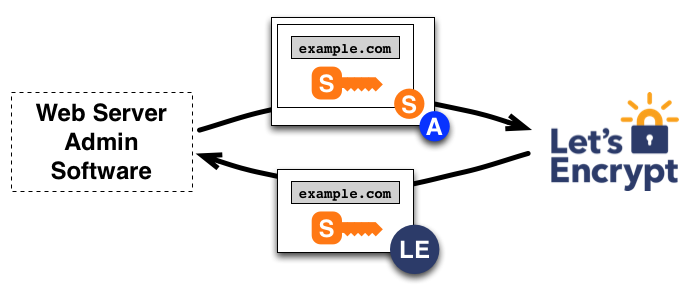
\includegraphics[width=65mm]{assets/official/letsencrypt-certificate.png}}
    \end{column}
  \end{columns}
  \DAsource{Let's Encrypt · How It Works}{https://letsencrypt.org/how-it-works/}
\end{frame}

\begin{frame}{8.7 HTTP-01 与 DNS-01 怎么选}{课堂单域名优先 HTTP-01}
  \begin{DAtable}{@{}p{25mm}p{44mm}p{51mm}@{}}
    \toprule
    验证方式 & 要求 & 适用 \\
    \midrule
    HTTP-01 & 域名已指向服务器，80 端口可访问 & 单域名、普通网站，配置简单 \\
    DNS-01 & 能通过 DNS 添加 TXT 记录 / API & 泛域名证书、80 不可达、集中证书管理 \\
    \bottomrule
  \end{DAtable}
  \begin{itemize}
    \item HTTP-01 申请失败先查 DNS、80 端口、防火墙和站点匹配。
    \item DNS API Token 使用最小权限，并像生产密钥一样保护。
  \end{itemize}
\end{frame}

\begin{frame}{8.8 宝塔申请与部署 SSL}{站点设置中完成申请、安装与续签}
  \begin{columns}[T]
    \begin{column}{0.50\textwidth}
      \centering
      \DAframed{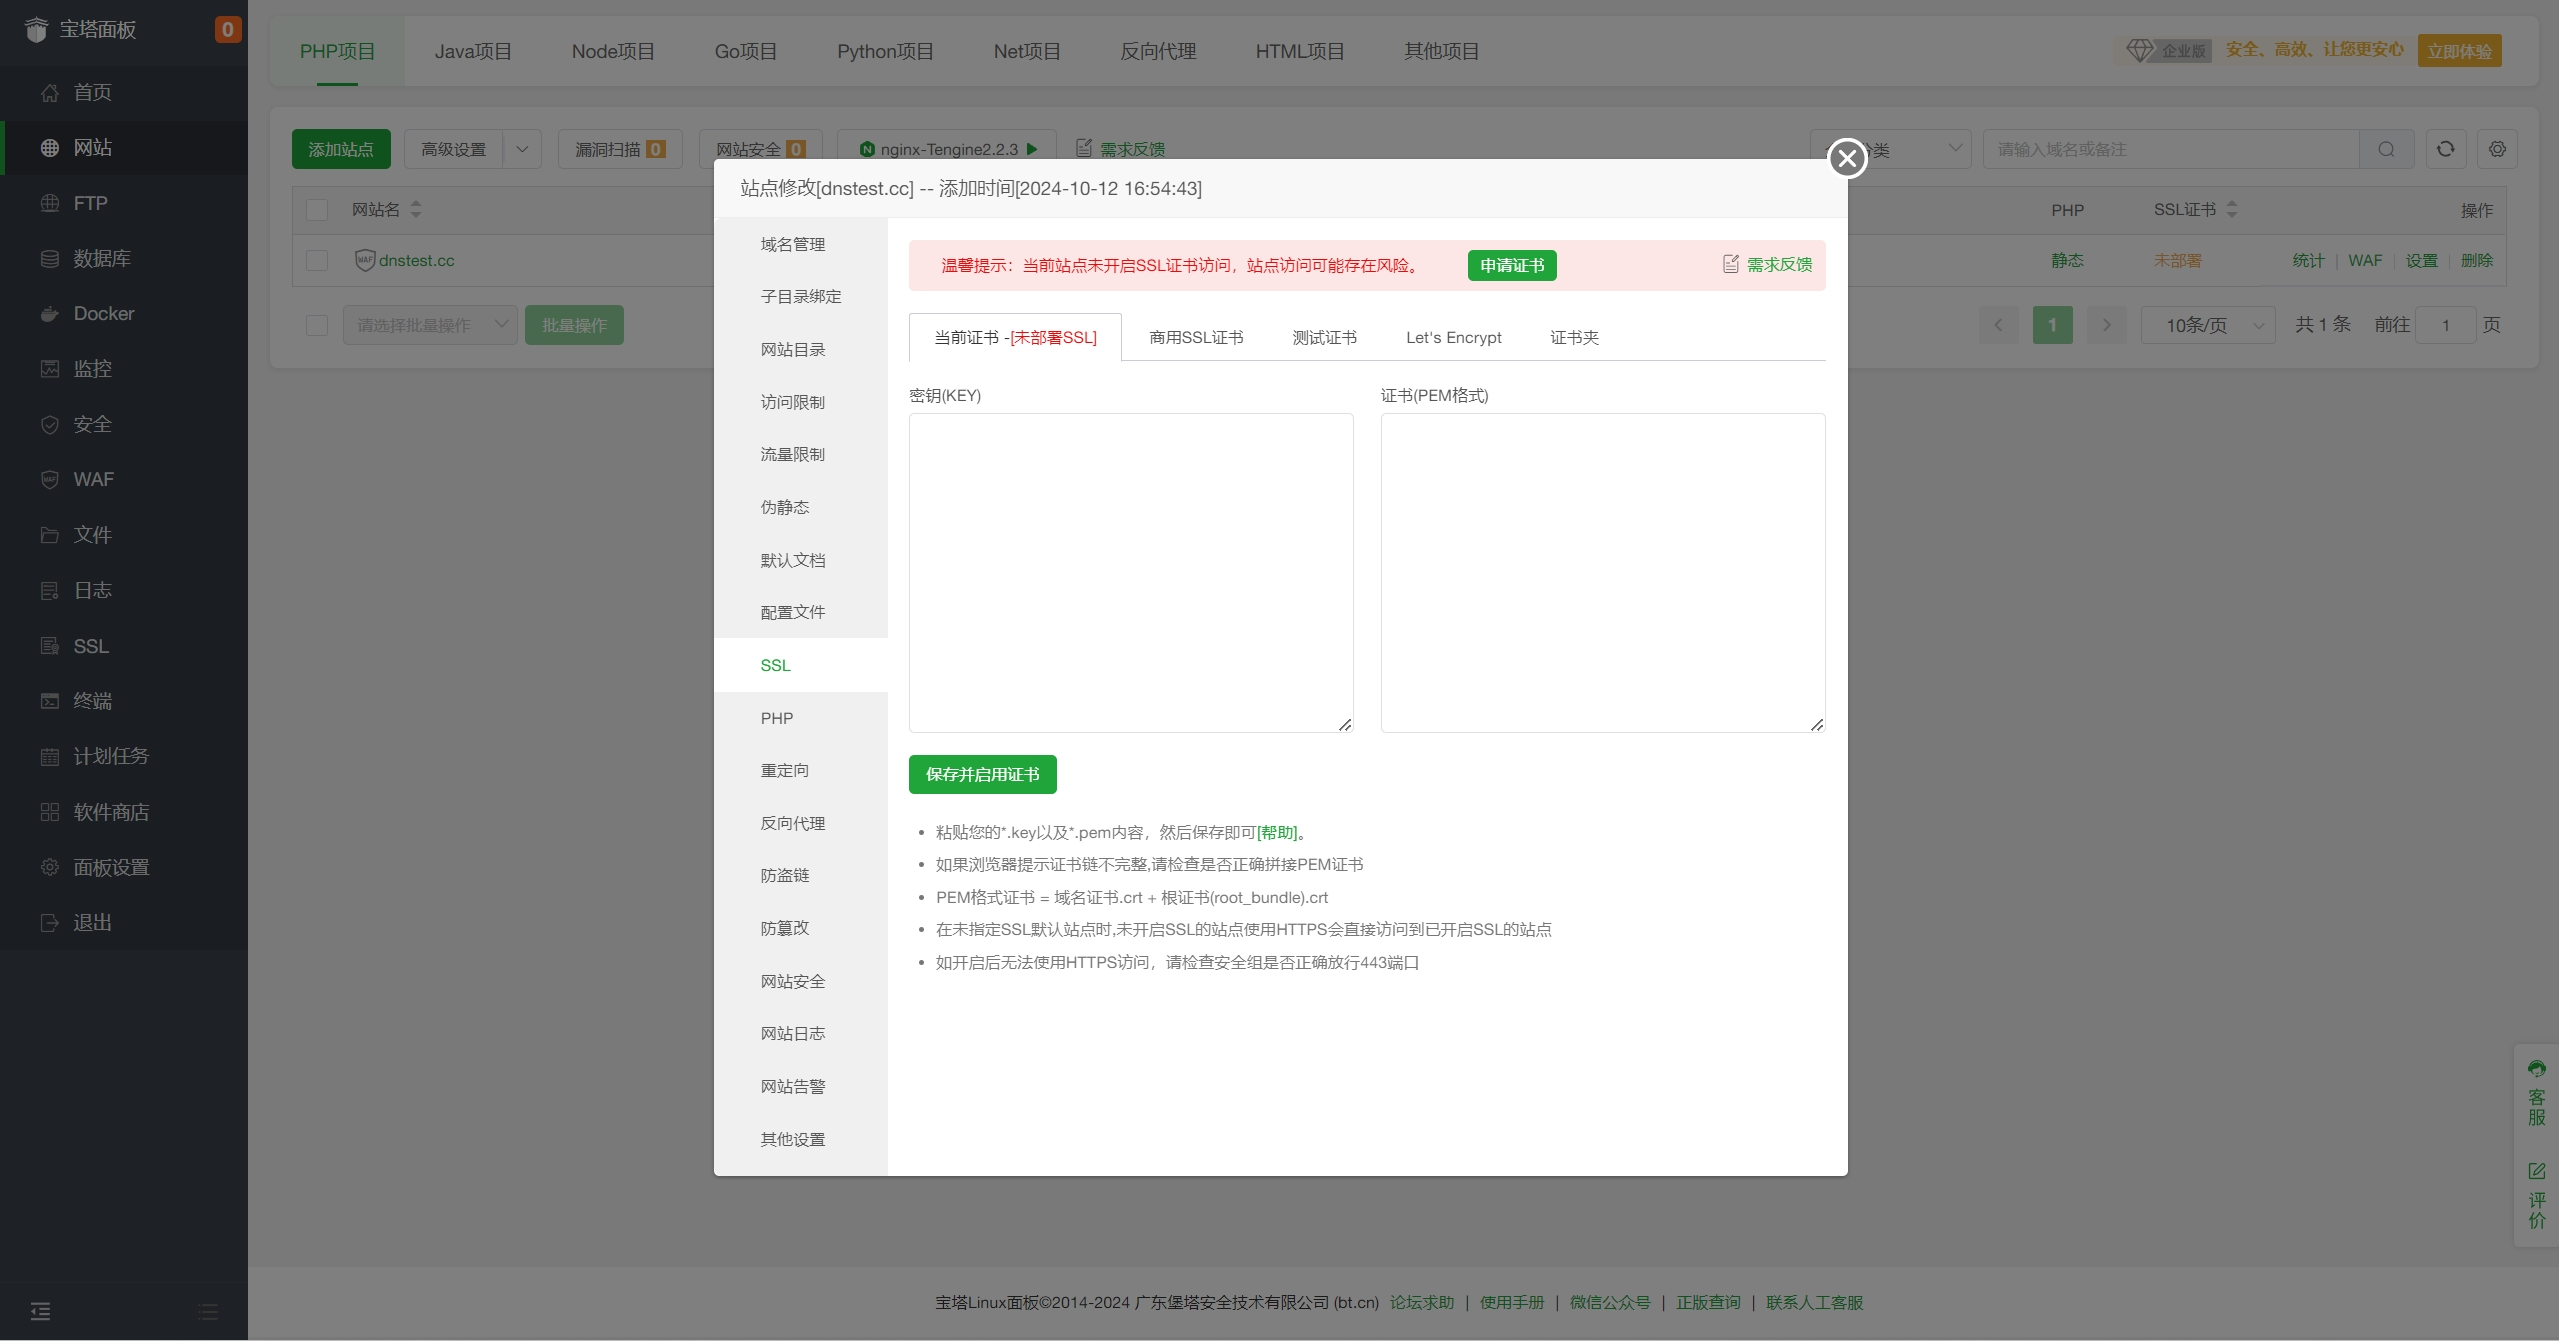
\includegraphics[height=39mm,trim=700 100 700 100,clip]{assets/official/bt-ssl.jpg}}
    \end{column}
    \begin{column}{0.46\textwidth}
      \begin{itemize}
        \item 域名先正确解析到服务器。
        \item 进入站点 SSL 页面申请。
        \item 可选免费证书或上传已有证书。
        \item 开启强制 HTTPS 与到期提醒。
      \end{itemize}
    \end{column}
  \end{columns}
  \DAsource{宝塔官方文档 · 部署 SSL 证书}{https://docs.bt.cn/getting-started/deploy-ssl}
\end{frame}

\begin{frame}[fragile]{8.9 HTTP 跳转 HTTPS}{80 端口保留验证与重定向}
  \begin{lstlisting}[language=bash]
server {
    listen 80;
    server_name app.example.com;

    location /.well-known/acme-challenge/ {
        root /www/server/panel/vhost/certbot;
    }

    location / {
        return 301 https://$host$request_uri;
    }
}
  \end{lstlisting}
  \begin{itemize}
    \item 宝塔通常会自动生成对应配置，不必手写路径。
    \item 强制 HTTPS 后，前端 API、图片、字体和 WebSocket 都应使用安全协议。
  \end{itemize}
\end{frame}

\begin{frame}{8.10 Mixed Content 排错}{HTTPS 页面中的 HTTP 请求会被拦截}
  \begin{alertblock}{典型错误}
    页面是 \DAfile{https://app.example.com}，前端仍请求 \DAfile{http://203.0.113.10:8000/api}。
  \end{alertblock}
  \begin{itemize}
    \item 浏览器会阻止不安全的 Fetch、XHR、Script、Stylesheet 等请求。
    \item 让 API、脚本、图片与 WebSocket 全部使用安全协议。
    \item 使用相对地址 \DAfile{/api}，可同时避免协议、域名与环境差异。
  \end{itemize}
  \DAsource{MDN · Mixed content}{https://developer.mozilla.org/en-US/docs/Web/Security/Defenses/Mixed_content}
\end{frame}

\begin{frame}{8.11 CORS 配置}{浏览器对跨 Origin 请求的约束}
  \begin{DAtable*}{@{}p{35mm}p{80mm}@{}}
    \toprule
    场景 & 处理 \\
    \midrule
    同域 \DAfile{/api} & 同源请求，配置最简 \\
    \DAfile{app.example.com} \(\rightarrow\) \DAfile{api.example.com} & 后端明确允许前端 Origin \\
    带 Cookie / Authorization & 不能用任意 \DAfile{*}；需精确 Origin 与 Credentials 配置 \\
    Postman / curl 能通，浏览器不通 & 优先检查 CORS 与 Preflight \\
    \bottomrule
  \end{DAtable*}
  \DAtagline{安全边界}{CORS 不能替代后端鉴权；攻击者可以不用浏览器直接请求 API}
\end{frame}

\begin{frame}[fragile]{8.12 上线后验证域名与证书}{检查跳转、证书、接口和安全头}
  \begin{lstlisting}[language=bash]
curl -I http://app.example.com
curl -I https://app.example.com
curl -i https://app.example.com/api/health

openssl s_client \
  -connect app.example.com:443 \
  -servername app.example.com </dev/null 2>/dev/null |
openssl x509 -noout -subject -issuer -dates
  \end{lstlisting}
  \begin{itemize}
    \item HTTP 应跳转 HTTPS；证书域名与有效期正确；API 返回预期 JSON。
    \item 浏览器控制台检查 Mixed Content、CORS、证书链与资源 404。
  \end{itemize}
\end{frame}

\begin{frame}{8.13 证书续签与 HSTS}{自动续签、到期提醒与安全策略}
  \begin{itemize}
    \item 免费证书通常周期较短，依赖自动续签；开启到期提醒。
    \item 续签失败常见原因：DNS 已切换、80 被关闭、验证路径被代理、DNS Token 失效。
    \item 确认 HTTPS 长期稳定后再考虑 HSTS。
    \item HSTS 配错会让浏览器拒绝回退 HTTP，证书错误时也无法绕过。
  \end{itemize}
  \DAtagline{运维要求}{持续监控自动续签与到期时间}
  \DAsource{MDN · Strict-Transport-Security}{https://developer.mozilla.org/en-US/docs/Web/HTTP/Reference/Headers/Strict-Transport-Security}
\end{frame}

\DAsection[日志、排错、备份、更新与恢复]{运维、排错、回滚与课堂实战}

\begin{frame}{9.1 线上故障按层定位}{从用户入口一路追到数据层}
  \centering
  \begin{tikzpicture}[node distance=2mm]
    \node[DAflow,minimum width=18mm] (dns) {DNS};
    \node[DAflow,minimum width=18mm,right=of dns] (tls) {TLS};
    \node[DAflow,minimum width=18mm,right=of tls] (nginx) {Nginx};
    \node[DAflow,minimum width=18mm,right=of nginx] (front) {Frontend};
    \node[DAflow,minimum width=18mm,right=of front] (api) {API};
    \node[DAflow,minimum width=18mm,right=of api] (db) {Database};
    \draw[DAarrowred] (dns) -- (tls);
    \draw[DAarrowred] (tls) -- (nginx);
    \draw[DAarrowred] (nginx) -- (front);
    \draw[DAarrowred] (front) -- (api);
    \draw[DAarrowred] (api) -- (db);
  \end{tikzpicture}
  \par\medskip
  \begin{itemize}
    \item 每层都用独立工具验证，找到“第一次失败”的位置。
    \item 页面报 500 时，从首次失败的层级开始处理。
  \end{itemize}
\end{frame}

\begin{frame}[fragile]{9.2 502 Bad Gateway 决策树}{Nginx 到上游的连接失败}
  \begin{lstlisting}[language=bash]
# 1. Is the process/container running?
docker compose ps
docker compose logs --tail 200 api

# 2. Is the port listening?
ss -lntp | grep 8000

# 3. Can the host/proxy reach it?
curl -i http://127.0.0.1:8000/health

# 4. Is Nginx config valid?
nginx -t
  \end{lstlisting}
  \DAtagline{结论}{本机 curl 都失败，先修应用；本机成功但域名失败，再查 Nginx 与防火墙}
\end{frame}

\begin{frame}{9.3 数据库连接失败怎么分层}{网络、账号、Schema、迁移}
  \begin{enumerate}
    \item 主机名是否正确：容器内用 \DAfile{db}，宿主机进程可能用 \DAfile{127.0.0.1}。
    \item 端口是否正确，数据库是否真正 Ready。
    \item 用户、密码、数据库名是否与初始化配置一致。
    \item 用户是否有目标数据库权限，字符集是否符合项目要求。
    \item 当前代码需要的迁移是否已执行。
  \end{enumerate}
  \DAtagline{容器陷阱}{API 容器里的 \DAfile{localhost:3306} 指向 API 容器自身}
\end{frame}

\begin{frame}[fragile]{9.4 服务器资源不足的症状}{构建时和运行时的瓶颈不同}
  \begin{lstlisting}[language=bash]
free -h
df -h
du -sh /var/lib/docker/*
docker stats
top
  \end{lstlisting}
  \begin{itemize}
    \item Node 前端构建常见内存峰值；MySQL、模型服务与多 Worker 会长期占内存。
    \item 磁盘可能被 Docker Image、Build Cache、日志和数据库共同吃满。
    \item OOM Kill 时应用像“突然消失”，需要查系统日志和容器退出码。
  \end{itemize}
\end{frame}

\begin{frame}{9.5 单机部署的安全基线}{默认拒绝，按需开放}
  \begin{columns}[T]
    \begin{column}{0.48\textwidth}
      \begin{itemize}
        \item SSH 使用密钥，限制 root 登录
        \item 面板入口限制来源并启用 HTTPS
        \item 公网只开放 22 / 80 / 443
        \item MySQL、Redis、API 端口不暴露公网
        \item 运行进程使用非 root 用户
      \end{itemize}
    \end{column}
    \begin{column}{0.48\textwidth}
      \begin{itemize}
        \item 系统与依赖定期更新
        \item Secret 最小权限并定期轮换
        \item 数据库与上传文件定期备份
        \item 日志与磁盘空间设告警
        \item 删除离职成员与过期 Deploy Key
      \end{itemize}
    \end{column}
  \end{columns}
  \DAtagline{现实边界}{一台服务器适合小型项目和教学；业务增长后再拆数据库、对象存储与负载均衡}
\end{frame}

\begin{frame}{9.6 一次规范发布包含哪些阶段}{发布前、中、后都要有证据}
  \begin{DAtable}{@{}p{23mm}p{94mm}@{}}
    \toprule
    阶段 & 动作 \\
    \midrule
    准备 & 分支已合并、测试通过、记录版本、备份、确认回滚点 \\
    构建 & 锁文件安装、生产构建、镜像打 Tag、扫描敏感信息 \\
    迁移 & 执行兼容性数据库迁移，失败则停止 \\
    发布 & 重启 / 替换进程或容器，保持变更范围最小 \\
    验证 & Health、首页、登录、数据库、关键 API、日志 \\
    观察 & 错误率、响应时间、资源、用户反馈 \\
    收尾 & 记录结果，删除临时权限，更新变更日志 \\
    \bottomrule
  \end{DAtable}
\end{frame}

\begin{frame}{9.7 回滚触发条件}{提前定义阈值与决策人}
  \begin{itemize}
    \item 健康检查持续失败，服务无法启动。
    \item 登录、支付、核心对话等关键链路不可用。
    \item 错误率或响应时间明显超过基线。
    \item 数据写入异常、权限越权、Secret 泄漏等安全事件。
    \item 修复时间不可控，继续在线排查会扩大影响。
  \end{itemize}
  \DAtagline{决策原则}{先恢复服务，再分析根因；回滚本身也需要验证与记录}
\end{frame}

\begin{frame}{9.8 从手工部署走向 CI/CD}{今天先把手工 SOP 做对，再自动化}
  \centering
  \begin{tikzpicture}[node distance=2mm]
    \node[DAflow,minimum width=18mm] (push) {Push / 合并};
    \node[DAflow,minimum width=18mm,right=of push] (ci) {CI\\Lint + Test};
    \node[DAflow,minimum width=18mm,right=of ci] (build) {Build\\Image + SHA};
    \node[DAflow,minimum width=18mm,right=of build] (registry) {Registry\\镜像};
    \node[DAflow,minimum width=18mm,right=of registry] (deploy) {Deploy\\Pull + Up};
    \node[DAflow,minimum width=18mm,right=of deploy] (verify) {Verify\\Smoke};
    \draw[DAarrowred] (push) -- (ci);
    \draw[DAarrowred] (ci) -- (build);
    \draw[DAarrowred] (build) -- (registry);
    \draw[DAarrowred] (registry) -- (deploy);
    \draw[DAarrowred] (deploy) -- (verify);
  \end{tikzpicture}
  \par\medskip
  \begin{itemize}
    \item 自动化把已验证的 SOP 固化为可重复流程。
    \item CI 使用与本地一致的 pnpm / uv 版本与锁文件策略。
  \end{itemize}
\end{frame}

\begin{frame}{9.9 课堂综合实战}{把 Day 3 / Day 4 项目真正交付给另一个人访问}
  \begin{enumerate}
    \item 确认上线前修复已经合并到主分支。
    \item 购买服务器后，完成宝塔基础环境配置。
    \item 选择宝塔手工路线或 Docker Compose 路线部署。
    \item 配置域名、\DAfile{/api} 反向代理与 SSL。
    \item 另一组使用手机网络访问并完成关键流程测试。
    \item 主动制造一次错误端口，按日志定位并恢复。
    \item 更新一个版本，再回滚到上一个版本。
  \end{enumerate}
\end{frame}

\begin{frame}{9.10 官方参考资料 · 宝塔、网络与 HTTPS}
  \scriptsize
  \begin{itemize}
    \item \href{https://docs.bt.cn/}{宝塔面板官方文档}
    \item \href{https://docs.bt.cn/user-guide/site/php/site-config/reverse-proxy}{宝塔 · 反向代理}
    \item \href{https://docs.bt.cn/getting-started/deploy-ssl}{宝塔 · 部署 SSL 证书}
    \item \href{https://docs.bt.cn/practical-tutorials/nodejs-pm2-deployment}{宝塔 · Node.js PM2 部署}
    \item \href{https://docs.nginx.com/nginx/admin-guide/web-server/reverse-proxy/}{NGINX Docs · Reverse Proxy}
    \item \href{https://developers.cloudflare.com/dns/}{Cloudflare Docs · DNS}
    \item \href{https://letsencrypt.org/how-it-works/}{Let's Encrypt · How It Works}
    \item \href{https://developer.mozilla.org/en-US/docs/Web/Security/Defenses/Mixed_content}{MDN · Mixed Content}
    \item \href{https://www.miit.gov.cn/}{工业和信息化部 · 互联网信息服务备案相关规定}
  \end{itemize}
\end{frame}


\DAclosing[交付完成]
\end{document}
